\PassOptionsToPackage{unicode=true}{hyperref} % options for packages loaded elsewhere
\PassOptionsToPackage{hyphens}{url}
%
\documentclass[]{book}
\usepackage{lmodern}
\usepackage{amssymb,amsmath}
\usepackage{ifxetex,ifluatex}
\usepackage{fixltx2e} % provides \textsubscript
\ifnum 0\ifxetex 1\fi\ifluatex 1\fi=0 % if pdftex
  \usepackage[T1]{fontenc}
  \usepackage[utf8]{inputenc}
  \usepackage{textcomp} % provides euro and other symbols
\else % if luatex or xelatex
  \usepackage{unicode-math}
  \defaultfontfeatures{Ligatures=TeX,Scale=MatchLowercase}
\fi
% use upquote if available, for straight quotes in verbatim environments
\IfFileExists{upquote.sty}{\usepackage{upquote}}{}
% use microtype if available
\IfFileExists{microtype.sty}{%
\usepackage[]{microtype}
\UseMicrotypeSet[protrusion]{basicmath} % disable protrusion for tt fonts
}{}
\IfFileExists{parskip.sty}{%
\usepackage{parskip}
}{% else
\setlength{\parindent}{0pt}
\setlength{\parskip}{6pt plus 2pt minus 1pt}
}
\usepackage{hyperref}
\hypersetup{
            pdftitle={Datenanalyse mit R},
            pdfauthor={Christina Bogner},
            pdfborder={0 0 0},
            breaklinks=true}
\urlstyle{same}  % don't use monospace font for urls
\usepackage{color}
\usepackage{fancyvrb}
\newcommand{\VerbBar}{|}
\newcommand{\VERB}{\Verb[commandchars=\\\{\}]}
\DefineVerbatimEnvironment{Highlighting}{Verbatim}{commandchars=\\\{\}}
% Add ',fontsize=\small' for more characters per line
\usepackage{framed}
\definecolor{shadecolor}{RGB}{248,248,248}
\newenvironment{Shaded}{\begin{snugshade}}{\end{snugshade}}
\newcommand{\AlertTok}[1]{\textcolor[rgb]{0.94,0.16,0.16}{#1}}
\newcommand{\AnnotationTok}[1]{\textcolor[rgb]{0.56,0.35,0.01}{\textbf{\textit{#1}}}}
\newcommand{\AttributeTok}[1]{\textcolor[rgb]{0.77,0.63,0.00}{#1}}
\newcommand{\BaseNTok}[1]{\textcolor[rgb]{0.00,0.00,0.81}{#1}}
\newcommand{\BuiltInTok}[1]{#1}
\newcommand{\CharTok}[1]{\textcolor[rgb]{0.31,0.60,0.02}{#1}}
\newcommand{\CommentTok}[1]{\textcolor[rgb]{0.56,0.35,0.01}{\textit{#1}}}
\newcommand{\CommentVarTok}[1]{\textcolor[rgb]{0.56,0.35,0.01}{\textbf{\textit{#1}}}}
\newcommand{\ConstantTok}[1]{\textcolor[rgb]{0.00,0.00,0.00}{#1}}
\newcommand{\ControlFlowTok}[1]{\textcolor[rgb]{0.13,0.29,0.53}{\textbf{#1}}}
\newcommand{\DataTypeTok}[1]{\textcolor[rgb]{0.13,0.29,0.53}{#1}}
\newcommand{\DecValTok}[1]{\textcolor[rgb]{0.00,0.00,0.81}{#1}}
\newcommand{\DocumentationTok}[1]{\textcolor[rgb]{0.56,0.35,0.01}{\textbf{\textit{#1}}}}
\newcommand{\ErrorTok}[1]{\textcolor[rgb]{0.64,0.00,0.00}{\textbf{#1}}}
\newcommand{\ExtensionTok}[1]{#1}
\newcommand{\FloatTok}[1]{\textcolor[rgb]{0.00,0.00,0.81}{#1}}
\newcommand{\FunctionTok}[1]{\textcolor[rgb]{0.00,0.00,0.00}{#1}}
\newcommand{\ImportTok}[1]{#1}
\newcommand{\InformationTok}[1]{\textcolor[rgb]{0.56,0.35,0.01}{\textbf{\textit{#1}}}}
\newcommand{\KeywordTok}[1]{\textcolor[rgb]{0.13,0.29,0.53}{\textbf{#1}}}
\newcommand{\NormalTok}[1]{#1}
\newcommand{\OperatorTok}[1]{\textcolor[rgb]{0.81,0.36,0.00}{\textbf{#1}}}
\newcommand{\OtherTok}[1]{\textcolor[rgb]{0.56,0.35,0.01}{#1}}
\newcommand{\PreprocessorTok}[1]{\textcolor[rgb]{0.56,0.35,0.01}{\textit{#1}}}
\newcommand{\RegionMarkerTok}[1]{#1}
\newcommand{\SpecialCharTok}[1]{\textcolor[rgb]{0.00,0.00,0.00}{#1}}
\newcommand{\SpecialStringTok}[1]{\textcolor[rgb]{0.31,0.60,0.02}{#1}}
\newcommand{\StringTok}[1]{\textcolor[rgb]{0.31,0.60,0.02}{#1}}
\newcommand{\VariableTok}[1]{\textcolor[rgb]{0.00,0.00,0.00}{#1}}
\newcommand{\VerbatimStringTok}[1]{\textcolor[rgb]{0.31,0.60,0.02}{#1}}
\newcommand{\WarningTok}[1]{\textcolor[rgb]{0.56,0.35,0.01}{\textbf{\textit{#1}}}}
\usepackage{longtable,booktabs}
% Fix footnotes in tables (requires footnote package)
\IfFileExists{footnote.sty}{\usepackage{footnote}\makesavenoteenv{longtable}}{}
\usepackage{graphicx,grffile}
\makeatletter
\def\maxwidth{\ifdim\Gin@nat@width>\linewidth\linewidth\else\Gin@nat@width\fi}
\def\maxheight{\ifdim\Gin@nat@height>\textheight\textheight\else\Gin@nat@height\fi}
\makeatother
% Scale images if necessary, so that they will not overflow the page
% margins by default, and it is still possible to overwrite the defaults
% using explicit options in \includegraphics[width, height, ...]{}
\setkeys{Gin}{width=\maxwidth,height=\maxheight,keepaspectratio}
\setlength{\emergencystretch}{3em}  % prevent overfull lines
\providecommand{\tightlist}{%
  \setlength{\itemsep}{0pt}\setlength{\parskip}{0pt}}
\setcounter{secnumdepth}{5}
% Redefines (sub)paragraphs to behave more like sections
\ifx\paragraph\undefined\else
\let\oldparagraph\paragraph
\renewcommand{\paragraph}[1]{\oldparagraph{#1}\mbox{}}
\fi
\ifx\subparagraph\undefined\else
\let\oldsubparagraph\subparagraph
\renewcommand{\subparagraph}[1]{\oldsubparagraph{#1}\mbox{}}
\fi

% set default figure placement to htbp
\makeatletter
\def\fps@figure{htbp}
\makeatother

\usepackage{booktabs}
\usepackage{amsthm}
\makeatletter
\def\thm@space@setup{%
  \thm@preskip=8pt plus 2pt minus 4pt
  \thm@postskip=\thm@preskip
}
\makeatother


\usepackage{xcolor}
\usepackage{mdframed}
\setlength{\fboxsep}{.8em}

%\definecolor{shadecolor}{rgb}{0.94, 0.97, 1.0}

\newenvironment{rmdinfo}{
  \definecolor{info}{rgb}{0.94, 0.97, 1.0}  %  	Alice blue
  \color{black}
  \begin{mdframed}[backgroundcolor = info]}
 {\end{mdframed}}

\newenvironment{rmdalert}{
  \definecolor{alert}{rgb}{0.96, 0.76, 0.76}  % babypink
  \color{black}
  \begin{mdframed}[backgroundcolor = alert]}
 {\end{mdframed}}


\newenvironment{rmdexample}{
  \definecolor{example}{rgb}{0.0, 0.8, 0.6}  % Caribbean green
  \color{black}
  \begin{mdframed}[backgroundcolor = example]}
 {\end{mdframed}}
 
 
\newenvironment{rmdoutcomes}{
  \definecolor{outcomes}{rgb}{1.0, 0.92, 0.8}  % Blanched Almond
  \color{black}
  \begin{mdframed}[backgroundcolor = outcomes]}
 {\end{mdframed}}

\newenvironment{rmdsummary}{
  \definecolor{summary}{rgb}{1.0, 0.8, 0.5}  % 
  \color{black}
  \begin{mdframed}[backgroundcolor = summary]}
 {\end{mdframed}}
\usepackage{etoolbox}
\makeatletter
\providecommand{\subtitle}[1]{% add subtitle to \maketitle
  \apptocmd{\@title}{\par {\large #1 \par}}{}{}
}
\makeatother
\usepackage[]{natbib}
\bibliographystyle{apalike}

\title{Datenanalyse mit R}
\providecommand{\subtitle}[1]{}
\subtitle{SoSe 2020}
\author{Christina Bogner}
\date{Version vom 04. Mai 2020}

\begin{document}
\maketitle

{
\setcounter{tocdepth}{1}
\tableofcontents
}
\hypertarget{vorwort}{%
\chapter{Vorwort}\label{vorwort}}

\begin{quote}
``And honey, we're gonna do it in style''
\end{quote}

\hfill --- Fools Garden

\hypertarget{organisatorisches}{%
\section{Organisatorisches}\label{organisatorisches}}

\begin{rmdinfo}
Die Coronaviruspandemie verändert unser Leben und unser Lernen. Die UzK
bittet Lehrende, zumindest zu Beginn des SoSe 2020 auf digitale
Lernformen umzusteigen. Daher wird dieser Kurs als ein Onlinekurs
beginnen. Abhängig von der (sehr dynamischen) Lage werden wir im
weiteren Kursverlauf das Format anpassen. Bitte seien Sie nachsichtig,
wenn nicht alles so klappt, wie in Präsenzveranstaltungen. Wir müssen
aktuell alle sehr viel dazu lernen in Sachen digitale Lehre. Sie können
sicher sein, dass das Geographische Institut bemüht ist, die Lehre so
effizient wie möglich weiter laufen zu lassen, damit Sie in Ihrem
Studium fortfahren können.
\end{rmdinfo}

In dieser Veranstaltung werden wir folgende Werkzeuge verwenden:

\begin{enumerate}
\def\labelenumi{\arabic{enumi}.}
\tightlist
\item
  \textbf{ILIAS}: die Online-Lernplattform der UzK. Entweder sind Sie bereits automatisch in dem Kurs registriert oder werden von mir per Hand angemeldet.
\item
  \textbf{Campuswire}: die Live-Chatplattform dient der allgemeinen Kommunikation und der Selbstorganisation des Lernens. Verwenden Sie diese, um Fragen mit Ihren Kommilitonen und mir zu diskutieren. Sie sollten eine Einladungsmail zu Campuswire erhalten haben.
\item
  \textbf{Zoom}: die Videokonferenz-Software werden wir für live Einführungen nutzen. Die Anmeldemodalitäten sind auf den Kursseiten in ILIAS erklärt.
\end{enumerate}

\hypertarget{sinn-und-unsinn-dieses-skripts}{%
\section{Sinn und Unsinn dieses Skripts}\label{sinn-und-unsinn-dieses-skripts}}

Dieses Skript ist ein lebendiges Begleitdokument des Kurses. Es wird laufend angepasst und aktualisiert.

Ich nutze verschiedene Farbkästen, um wichtige Stellen hervorzuheben:

\begin{rmdinfo}
Infoblock
\end{rmdinfo}

\begin{rmdalert}
Achtung, wichtig!
\end{rmdalert}

\begin{rmdexample}
Beispielblock
\end{rmdexample}

\begin{rmdoutcomes}
Lernziele
\end{rmdoutcomes}

\begin{rmdsummary}
Zusammenfassung
\end{rmdsummary}

\hypertarget{einfuehrung}{%
\chapter{Der Kurs}\label{einfuehrung}}

\hypertarget{zuordnung-zum-modul-und-leistungsnachweis}{%
\section{Zuordnung zum Modul und Leistungsnachweis}\label{zuordnung-zum-modul-und-leistungsnachweis}}

Dieser Kurs gehört zum Modul \emph{Fachmethodik I} oder \emph{Fachmethodik II} und ist aus 4 SWS Praktikum und 2 SWS Seminar aufgebaut. Das wichtigste Ziel besteht darin, Ihnen einen sicheren Umgang mit \texttt{R} beizubringen.

Den Leistungsnachweis bildet ein benoteter Praktikumsbericht.

\hypertarget{lernziele-des-kurses}{%
\section{Lernziele des Kurses}\label{lernziele-des-kurses}}

\begin{rmdoutcomes}
\begin{itemize}
\tightlist
\item
  Daten für Analysen vorbereiten
\item
  eigene wiederverwendbare Skripte schreiben
\item
  eigene Funktionen schreiben
\item
  einfache Datenanalysen durchführen
\item
  Daten visualisieren
\item
  Ergebnisse reproduzierbar im Praktikumsbericht darstellen
\end{itemize}
\end{rmdoutcomes}

\hypertarget{was-mir-im-umgang-miteinander-wichtig-ist}{%
\section{Was mir im Umgang miteinander wichtig ist}\label{was-mir-im-umgang-miteinander-wichtig-ist}}

\begin{itemize}
\tightlist
\item
  Pünktlichkeit bei live und Präsenzsitzungen
\item
  Gute Vorbereitung durch erledigen der blenden learning Einheiten und Hausaufgaben
\item
  Respektieren anderer Meinungen
\item
  Offenheit gegenüber neuen Sichtweisen, Themen und Methoden
\item
  Geduld mit sich selbst und den anderen 😄
\end{itemize}

\hypertarget{erste_schritte}{%
\chapter{Erste Schritte in }\label{erste_schritte}}

\begin{rmdoutcomes}
\begin{itemize}
\tightlist
\item
  Layout und Bedeutung einzelner Fenster in RStudio kennen
\item
  Anweisungen aus dem Skript an die Konsole schicken
\item
  R als Taschenrechner benutzen
\item
  erste Funktionen aufrufen
\item
  Objekte mit eckigen Klammern {[} {]} ansprechen
\item
  R-Hilfeseiten aufrufen
\end{itemize}
\end{rmdoutcomes}

\hypertarget{was-ist-r}{%
\section{Was ist R?}\label{was-ist-r}}

R ist eine Programmiersprache für Datenanalyse und statistische Modellierung. Es ist frei verfügbar (\emph{open source software}) und neben Python einer der am meisten benutzten Programmiersprachen zur Datenanalyse und -visualisierung. R wurde von Ross Ihaka und Robert Gentleman 1996 veröffentlicht \citet{Ihaka1996}. Es gibt für R eine Vielzahl von Zusatzpaketen, die die Funktionalität und die Einsatzmöglichkeiten enorm erweitern.

Sie können R für Ihren Computer auf der offiziellen R-Seite \url{https://www.r-project.org/} herunter laden und installieren. Auch die Pakete finden Sie dort unter CRAN (\emph{The Comprehensive R Archive Network}). Auf den CRAN-Seiten finden Sie sogen. \href{http://cran.r-project.org/web/views/}{CRAN Task Views}, eine Übersicht über Pakete in verschiedenen Themenbereichen. Für den Umweltbereich sind folgende Paketsammlungen besonders relevant:

\begin{itemize}
\tightlist
\item
  Environmetrics: Analyse von Umweltdaten
\item
  Multivariate: Multivariate Statistik
\item
  Spatial: Analyse von räumlichen Daten
\item
  TimeSeries: Zeitreihenanalyse
\end{itemize}

Zu Beginn des Kurses, werden wir jedoch nicht auf Ihren lokalen Rechnern arbeiten, sondern in einer Cloud (s.u.). Das ermöglicht einen schnelleren Einstieg in R und bietet eine live Unterstützung durch den Dozenten beim Programmieren. Daher biete ich zu diesem frühen Zeitpunkt im Kurs keine Unterstützung bei der Installation. Für die ganz Ungeduldigen, gibt es hier eine kurze \emph{Einleitung zur Installation}

\hypertarget{was-ist-rstudio}{%
\section{Was ist RStudio?}\label{was-ist-rstudio}}

RStudio Desktop ist eine Entwicklungsumgebung für R. Sie können die \emph{open source} Version kostenlos für Ihren Rechner \href{https://rstudio.com/products/rstudio/\#rstudio-desktop}{hier} herunterladen.

Es gibt eine live Einführung in RStudio im Kurs. Zusätzlich können Sie hier ein Video dazu ansehen.

\hypertarget{rstudio-cloud}{%
\section{RStudio Cloud}\label{rstudio-cloud}}

Zu Beginn des Kurses werden wir in der \href{https://rstudio.cloud/}{RStudio Cloud} arbeiten. Sie sollten eine Einladungsmail zu unserem Kurs in der Cloud bekommen haben. Ich werde in der Cloud Projekte für Sie anlegen (\emph{assignment}), die Skripte, Arbeitsanweisungen etc. beinhalten. Wenn Sie auf so ein Assignment klicken, wird für Sie automatische ein Kopie des Projekts erstellt, in der Sie dann arbeiten können.

Der große Vorteil der Cloud ist, dass ich direkt in Ihre Projekte eingreifen kann, wenn es mal zu Fehlern kommt. Während ich in Ihrem Projekt arbeite, werden Sie kurz aus der R-Sitzung ausgeloggt, da die Cloud kein gleichzeitiges Arbeiten unterstützt. Nehmen Sie sich etwas Zeit, um die Cloud und die darin enthaltenen \href{https://rstudio.cloud/learn/primers}{Tutorials} kennen zu lernen.

Sowohl in der RStudio Cloud als auch in einer lokalen Installation, ist Ihr RStudio so aufgebaut wie in Abbildung \ref{fig:rstudio}.

\begin{figure}
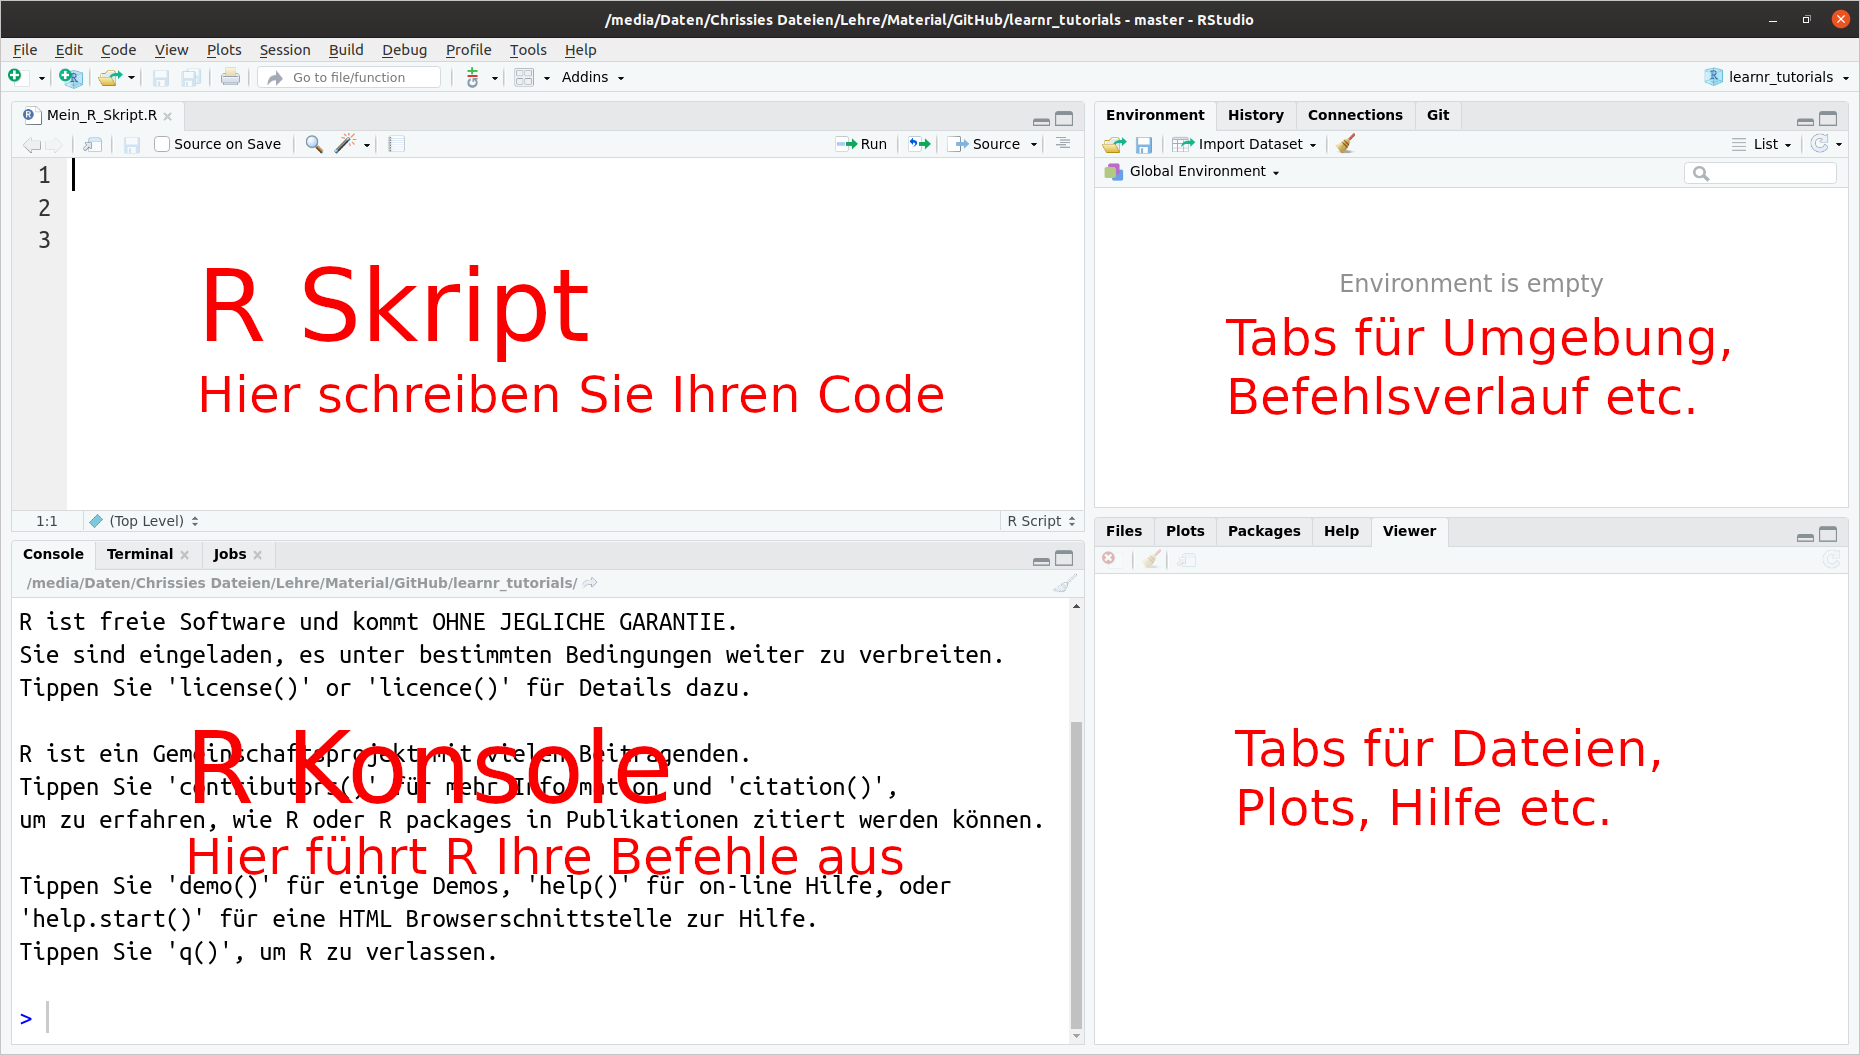
\includegraphics[width=1\linewidth]{RStudio} \caption{Aufbau von RStudio}\label{fig:rstudio}
\end{figure}

\hypertarget{inhalt-der-live-einfuxfchrung}{%
\section{Inhalt der live Einführung}\label{inhalt-der-live-einfuxfchrung}}

\begin{itemize}
\tightlist
\item
  Überblick über RStudio
\item
  R als Taschenrechner
\item
  einfache Funktionen aufrufen
\item
  Zuordnungen (\emph{assignments})
\item
  Notation mit eckigen Klammern {[} {]} (\emph{array}-Notation)
\item
  Hilfeseiten aufrufen
\end{itemize}

Funktionen, die wir in der Session nutzen werden:

\begin{longtable}[]{@{}lll@{}}
\toprule
\begin{minipage}[b]{0.30\columnwidth}\raggedright
Funktion\strut
\end{minipage} & \begin{minipage}[b]{0.28\columnwidth}\raggedright
Bedeutung\strut
\end{minipage} & \begin{minipage}[b]{0.33\columnwidth}\raggedright
Beispielaufruf\strut
\end{minipage}\tabularnewline
\midrule
\endhead
\begin{minipage}[t]{0.30\columnwidth}\raggedright
\texttt{pi}\strut
\end{minipage} & \begin{minipage}[t]{0.28\columnwidth}\raggedright
Zahl pi\strut
\end{minipage} & \begin{minipage}[t]{0.33\columnwidth}\raggedright
\texttt{pi}\strut
\end{minipage}\tabularnewline
\begin{minipage}[t]{0.30\columnwidth}\raggedright
\texttt{sin}\strut
\end{minipage} & \begin{minipage}[t]{0.28\columnwidth}\raggedright
Sinus\strut
\end{minipage} & \begin{minipage}[t]{0.33\columnwidth}\raggedright
\texttt{sin(2)}\strut
\end{minipage}\tabularnewline
\begin{minipage}[t]{0.30\columnwidth}\raggedright
\texttt{cos}\strut
\end{minipage} & \begin{minipage}[t]{0.28\columnwidth}\raggedright
Cosinus\strut
\end{minipage} & \begin{minipage}[t]{0.33\columnwidth}\raggedright
\texttt{cos(2)}\strut
\end{minipage}\tabularnewline
\begin{minipage}[t]{0.30\columnwidth}\raggedright
\texttt{sqrt}\strut
\end{minipage} & \begin{minipage}[t]{0.28\columnwidth}\raggedright
Quadratwurzel\strut
\end{minipage} & \begin{minipage}[t]{0.33\columnwidth}\raggedright
\texttt{sqrt(2)}\strut
\end{minipage}\tabularnewline
\begin{minipage}[t]{0.30\columnwidth}\raggedright
\texttt{c}\strut
\end{minipage} & \begin{minipage}[t]{0.28\columnwidth}\raggedright
(\emph{concatenate}) Fügt Daten zu einem Vektor zusammen\strut
\end{minipage} & \begin{minipage}[t]{0.33\columnwidth}\raggedright
\texttt{c(1,2,3,4)}\strut
\end{minipage}\tabularnewline
\begin{minipage}[t]{0.30\columnwidth}\raggedright
\texttt{help.start}\strut
\end{minipage} & \begin{minipage}[t]{0.28\columnwidth}\raggedright
Öffnet ein Browser-Fenster mit diversen Handbüchern\strut
\end{minipage} & \begin{minipage}[t]{0.33\columnwidth}\raggedright
\texttt{help.start()}\strut
\end{minipage}\tabularnewline
\begin{minipage}[t]{0.30\columnwidth}\raggedright
\texttt{help.search}\strut
\end{minipage} & \begin{minipage}[t]{0.28\columnwidth}\raggedright
Sucht nach einem Begriff in Hilfe-Dateien\strut
\end{minipage} & \begin{minipage}[t]{0.33\columnwidth}\raggedright
\texttt{help.search(\textquotesingle{}time\textquotesingle{})}\strut
\end{minipage}\tabularnewline
\begin{minipage}[t]{0.30\columnwidth}\raggedright
\texttt{??}\strut
\end{minipage} & \begin{minipage}[t]{0.28\columnwidth}\raggedright
alias \texttt{help.search}\strut
\end{minipage} & \begin{minipage}[t]{0.33\columnwidth}\raggedright
\texttt{??time}\strut
\end{minipage}\tabularnewline
\begin{minipage}[t]{0.30\columnwidth}\raggedright
\texttt{help}\strut
\end{minipage} & \begin{minipage}[t]{0.28\columnwidth}\raggedright
Sucht nach einer Funktion\strut
\end{minipage} & \begin{minipage}[t]{0.33\columnwidth}\raggedright
\texttt{?mean}\strut
\end{minipage}\tabularnewline
\begin{minipage}[t]{0.30\columnwidth}\raggedright
\texttt{?}\strut
\end{minipage} & \begin{minipage}[t]{0.28\columnwidth}\raggedright
alias \texttt{help()}\strut
\end{minipage} & \begin{minipage}[t]{0.33\columnwidth}\raggedright
\texttt{?mean}\strut
\end{minipage}\tabularnewline
\begin{minipage}[t]{0.30\columnwidth}\raggedright
\texttt{mean}\strut
\end{minipage} & \begin{minipage}[t]{0.28\columnwidth}\raggedright
Mittelwert\strut
\end{minipage} & \begin{minipage}[t]{0.33\columnwidth}\raggedright
\texttt{mean(c(1,2,3,4))}\strut
\end{minipage}\tabularnewline
\begin{minipage}[t]{0.30\columnwidth}\raggedright
\texttt{var}\strut
\end{minipage} & \begin{minipage}[t]{0.28\columnwidth}\raggedright
Varianz\strut
\end{minipage} & \begin{minipage}[t]{0.33\columnwidth}\raggedright
\texttt{var(c(1,2,3,4))}\strut
\end{minipage}\tabularnewline
\begin{minipage}[t]{0.30\columnwidth}\raggedright
\texttt{sd}\strut
\end{minipage} & \begin{minipage}[t]{0.28\columnwidth}\raggedright
Standardabweichung\strut
\end{minipage} & \begin{minipage}[t]{0.33\columnwidth}\raggedright
\texttt{sd(c(1,2,3,4))}\strut
\end{minipage}\tabularnewline
\begin{minipage}[t]{0.30\columnwidth}\raggedright
\texttt{sum}\strut
\end{minipage} & \begin{minipage}[t]{0.28\columnwidth}\raggedright
Summe\strut
\end{minipage} & \begin{minipage}[t]{0.33\columnwidth}\raggedright
\texttt{sum(c(1,2,3,4))}\strut
\end{minipage}\tabularnewline
\begin{minipage}[t]{0.30\columnwidth}\raggedright
\texttt{vector}\strut
\end{minipage} & \begin{minipage}[t]{0.28\columnwidth}\raggedright
Generiert einen Vektor\strut
\end{minipage} & \begin{minipage}[t]{0.33\columnwidth}\raggedright
\texttt{vector(length=3,\ mode=\textquotesingle{}numeric\textquotesingle{})}\strut
\end{minipage}\tabularnewline
\bottomrule
\end{longtable}

\hypertarget{daten}{%
\chapter{Daten in R}\label{daten}}

\begin{rmdoutcomes}
\begin{itemize}
\tightlist
\item
  Daten einlesen mit \texttt{read.table}
\item
  Datenstrukturen erstellen
\item
  Typen von Daten in R abfragen
\item
  Daten speichern mit \texttt{write.table}
\end{itemize}
\end{rmdoutcomes}

\hypertarget{datenstrukturen-erzeugen}{%
\section{Datenstrukturen erzeugen}\label{datenstrukturen-erzeugen}}

In R gibt es unterschiedliche Datenobjekte. Es ist wichtig, sich über die Struktur (oder Typ) des Datenobjekts Gedanken zu machen. Denn diese bestimmt, was mit einem Objekt gemacht werden kann und ob Funktionen damit richtig umgehen können. Schließlich ist es nicht egal, ob es sich bei einem Objekt um ein numerisches Objekt oder einfach Text (\emph{character}) handelt.

Die wichtigsten Datentypen sind

\begin{itemize}
\tightlist
\item
  \textbf{Vektoren}: hier gruppiert man gleichartige Elemente, z.B. Zahlen. Auch eine einzelne Zahl (ein Skalar) wird von R wie ein Vektor behandelt.
\item
  \textbf{Matrizen}: zweidimensionale (Zeilen und Spalten) Datentabellen mit gleichartigen Elementen.
\item
  \textbf{Listen}: können beliebige Elemente beliebiger Länge enthalten.
\item
  \textbf{Dataframes}: zweidimensionale Datentabellen, die beliebige Elemente enthalten können. Die Spalten der Dataframes müssen allerdings gleichartige Elemente enthalten. Dataframes sind eine Unterart von Listen.
\end{itemize}

Neben diesen Hauptstrukturen gibt es

\begin{itemize}
\tightlist
\item
  \textbf{Factor}: ein besonderer Vektor für kategorielle Variablen
\end{itemize}

Um diese Datenstrukturen zu erzeugen, gibt es jeweils eine Funktion mit gleichlautendem Namen.

\begin{Shaded}
\begin{Highlighting}[]
\CommentTok{# Vektor erzeugen}
\NormalTok{my_vect =}\StringTok{ }\KeywordTok{vector}\NormalTok{(}\DataTypeTok{length =} \DecValTok{3}\NormalTok{, }\DataTypeTok{mode =} \StringTok{'numeric'}\NormalTok{)}
\NormalTok{my_vect}
\end{Highlighting}
\end{Shaded}

\begin{verbatim}
## [1] 0 0 0
\end{verbatim}

\begin{Shaded}
\begin{Highlighting}[]
\CommentTok{# Matrix erzeugen}
\NormalTok{my_matrix =}\StringTok{ }\KeywordTok{matrix}\NormalTok{(}\DataTypeTok{data =} \KeywordTok{c}\NormalTok{(}\DecValTok{1}\OperatorTok{:}\NormalTok{(}\DecValTok{3}\OperatorTok{*}\DecValTok{4}\NormalTok{)), }\DataTypeTok{nrow =} \DecValTok{3}\NormalTok{, }\DataTypeTok{ncol =} \DecValTok{4}\NormalTok{)}
\NormalTok{my_matrix}
\end{Highlighting}
\end{Shaded}

\begin{verbatim}
##      [,1] [,2] [,3] [,4]
## [1,]    1    4    7   10
## [2,]    2    5    8   11
## [3,]    3    6    9   12
\end{verbatim}

\begin{Shaded}
\begin{Highlighting}[]
\CommentTok{# Dataframe erzeugen}
\NormalTok{my_dataframe =}\StringTok{ }\KeywordTok{data.frame}\NormalTok{(}\StringTok{'Spalte_1'}\NormalTok{ =}\StringTok{ }\KeywordTok{rep}\NormalTok{(}\StringTok{'Text'}\NormalTok{, }\DecValTok{10}\NormalTok{),}
                          \StringTok{'Spalte_2'}\NormalTok{ =}\StringTok{ }\DecValTok{1}\OperatorTok{:}\DecValTok{10}\NormalTok{)}
\NormalTok{my_dataframe}
\end{Highlighting}
\end{Shaded}

\begin{verbatim}
##    Spalte_1 Spalte_2
## 1      Text        1
## 2      Text        2
## 3      Text        3
## 4      Text        4
## 5      Text        5
## 6      Text        6
## 7      Text        7
## 8      Text        8
## 9      Text        9
## 10     Text       10
\end{verbatim}

\begin{Shaded}
\begin{Highlighting}[]
\CommentTok{# Liste erzeugen}
\NormalTok{my_list =}\StringTok{ }\KeywordTok{list}\NormalTok{(}\StringTok{'Schachtel_1'}\NormalTok{ =}\StringTok{ }\DecValTok{3}\NormalTok{, }\StringTok{'Schachtel_2'}\NormalTok{ =}\StringTok{ }\NormalTok{my_dataframe,}
               \StringTok{'Schachtel_3'}\NormalTok{ =}\StringTok{ 'Noch mehr Text'}\NormalTok{)}
\NormalTok{my_list}
\end{Highlighting}
\end{Shaded}

\begin{verbatim}
## $Schachtel_1
## [1] 3
## 
## $Schachtel_2
##    Spalte_1 Spalte_2
## 1      Text        1
## 2      Text        2
## 3      Text        3
## 4      Text        4
## 5      Text        5
## 6      Text        6
## 7      Text        7
## 8      Text        8
## 9      Text        9
## 10     Text       10
## 
## $Schachtel_3
## [1] "Noch mehr Text"
\end{verbatim}

\begin{Shaded}
\begin{Highlighting}[]
\CommentTok{# Factor erzeugen}
\NormalTok{my_factor =}\StringTok{ }\KeywordTok{factor}\NormalTok{(}\KeywordTok{c}\NormalTok{(}\StringTok{'R'}\NormalTok{, }\StringTok{'RStudio'}\NormalTok{, }\StringTok{'Cloud'}\NormalTok{, }\StringTok{'Cloud'}\NormalTok{, }\StringTok{'R'}\NormalTok{, }\StringTok{'R'}\NormalTok{))}
\NormalTok{my_factor}
\end{Highlighting}
\end{Shaded}

\begin{verbatim}
## [1] R       RStudio Cloud   Cloud   R       R      
## Levels: Cloud R RStudio
\end{verbatim}

\hypertarget{arten-von-daten-in-r}{%
\section{Arten von Daten in R}\label{arten-von-daten-in-r}}

Die Datenstrukturen \texttt{vector}, \texttt{data.frame} usw. können unterschiedliche Arten von Daten enthalten.

\begin{longtable}[]{@{}ll@{}}
\toprule
Name & Beispiele\tabularnewline
\midrule
\endhead
raw & 3A, FE\tabularnewline
logical & TRUE, FALSE\tabularnewline
integer & 1, 42, -3\tabularnewline
numeric/double & 3, 2.81, 6.032e23\tabularnewline
complex & 1.2+2.2i\tabularnewline
character & ``foo''\tabularnewline
\bottomrule
\end{longtable}

\hypertarget{objekt-sag-mir-wer-du-bist}{%
\section{Objekt, sag mir wer du bist}\label{objekt-sag-mir-wer-du-bist}}

Um die Struktur und/oder Datenart abzufragen, verwendet man \texttt{class}, \texttt{typeof}, \texttt{mode} und \texttt{storage.mode}.

\begin{Shaded}
\begin{Highlighting}[]
\KeywordTok{class}\NormalTok{(my_vect)}
\end{Highlighting}
\end{Shaded}

\begin{verbatim}
## [1] "numeric"
\end{verbatim}

\begin{Shaded}
\begin{Highlighting}[]
\KeywordTok{typeof}\NormalTok{(my_vect)}
\end{Highlighting}
\end{Shaded}

\begin{verbatim}
## [1] "double"
\end{verbatim}

\begin{Shaded}
\begin{Highlighting}[]
\KeywordTok{class}\NormalTok{(my_dataframe)}
\end{Highlighting}
\end{Shaded}

\begin{verbatim}
## [1] "data.frame"
\end{verbatim}

\begin{Shaded}
\begin{Highlighting}[]
\KeywordTok{typeof}\NormalTok{(my_dataframe)}
\end{Highlighting}
\end{Shaded}

\begin{verbatim}
## [1] "list"
\end{verbatim}

Mit \texttt{str} kann man das Innenleben eines Objekts anzeigen. Das ist besonders wichtig nach dem Einlesen von Daten, um das Ergebnis des Einlesens zu kontrollieren. Dabei kontrolliert man, dass z.B. alle numerischen Spalten auch als Zahlen eingelesen wurden und nichts schief gegangen ist.

\begin{Shaded}
\begin{Highlighting}[]
\KeywordTok{str}\NormalTok{(my_dataframe)}
\end{Highlighting}
\end{Shaded}

\begin{verbatim}
## 'data.frame':    10 obs. of  2 variables:
##  $ Spalte_1: Factor w/ 1 level "Text": 1 1 1 1 1 1 1 1 1 1
##  $ Spalte_2: int  1 2 3 4 5 6 7 8 9 10
\end{verbatim}

Weiter Funktionen, die Auskunft über Objekte geben sind \texttt{length}, sinnvoll auf nur Vektoren und Listen, und \texttt{dim}, sinnvoll auf zweidimensionalen Datenobjekten. Wenn Sie versuchen, \texttt{dim} auf einem Vektor aufzurufen, gibt es \texttt{NULL} (s.u.), weil Vektoren keine Dimensionen haben. Wenn Sie \texttt{length} auf einem \texttt{data.frame} aufrufen, bekommen Sie die Anzahl der Dimensionen, nämlich 2. Das sind keine besonders spannenden Informationen 😄.

\begin{Shaded}
\begin{Highlighting}[]
\KeywordTok{length}\NormalTok{(my_vect)}
\end{Highlighting}
\end{Shaded}

\begin{verbatim}
## [1] 3
\end{verbatim}

\begin{Shaded}
\begin{Highlighting}[]
\KeywordTok{dim}\NormalTok{(my_vect)}
\end{Highlighting}
\end{Shaded}

\begin{verbatim}
## NULL
\end{verbatim}

\begin{Shaded}
\begin{Highlighting}[]
\KeywordTok{length}\NormalTok{(my_dataframe)}
\end{Highlighting}
\end{Shaded}

\begin{verbatim}
## [1] 2
\end{verbatim}

\begin{Shaded}
\begin{Highlighting}[]
\KeywordTok{dim}\NormalTok{(my_dataframe)}
\end{Highlighting}
\end{Shaded}

\begin{verbatim}
## [1] 10  2
\end{verbatim}

\hypertarget{datenluxfccken-fehlschluxe4ge-etc.}{%
\section{Datenlücken, Fehlschläge etc.}\label{datenluxfccken-fehlschluxe4ge-etc.}}

Datenlücken werden in R mit \texttt{NA} kodiert, Fehlschläge bei Berechnungen mit \texttt{NaN} (not a number) und Vektoren der Länge 0 mit \texttt{NULL}. Letzteres wird häufig beim Aufruf von Funktionen benutzt, wenn man bestimmte Parameter ausschalten möchte. Die Benutzung muss aber immer in der Hilfe zur jeweiligen Funktion nachgeschlagen werden.

\hypertarget{inhalt-der-live-einfuxfchrung-1}{%
\section{Inhalt der live Einführung}\label{inhalt-der-live-einfuxfchrung-1}}

\begin{itemize}
\tightlist
\item
  Daten einlesen und \texttt{data.frame} erstellen: Aufgabe \ref{bestandesaufnahme}
\end{itemize}

Funktionen, die wir in der Session nutzen werden:

\begin{longtable}[]{@{}lll@{}}
\toprule
\begin{minipage}[b]{0.30\columnwidth}\raggedright
Funktion\strut
\end{minipage} & \begin{minipage}[b]{0.28\columnwidth}\raggedright
Bedeutung\strut
\end{minipage} & \begin{minipage}[b]{0.33\columnwidth}\raggedright
Beispielaufruf\strut
\end{minipage}\tabularnewline
\midrule
\endhead
\begin{minipage}[t]{0.30\columnwidth}\raggedright
\texttt{read.table}\strut
\end{minipage} & \begin{minipage}[t]{0.28\columnwidth}\raggedright
Liest Daten aus einer Datei ein.\strut
\end{minipage} & \begin{minipage}[t]{0.33\columnwidth}\raggedright
\texttt{read.table(file=\ \textquotesingle{}Daten.txt\textquotesingle{},\ header=TRUE)}\strut
\end{minipage}\tabularnewline
\begin{minipage}[t]{0.30\columnwidth}\raggedright
\texttt{ls}\strut
\end{minipage} & \begin{minipage}[t]{0.28\columnwidth}\raggedright
Zeigt den Inhalt des Workspaces.\strut
\end{minipage} & \begin{minipage}[t]{0.33\columnwidth}\raggedright
\texttt{ls}\strut
\end{minipage}\tabularnewline
\begin{minipage}[t]{0.30\columnwidth}\raggedright
\texttt{head}\strut
\end{minipage} & \begin{minipage}[t]{0.28\columnwidth}\raggedright
Zeigt den ersten Teil eines Objekts.\strut
\end{minipage} & \begin{minipage}[t]{0.33\columnwidth}\raggedright
\texttt{head(x)}\strut
\end{minipage}\tabularnewline
\begin{minipage}[t]{0.30\columnwidth}\raggedright
\texttt{tail}\strut
\end{minipage} & \begin{minipage}[t]{0.28\columnwidth}\raggedright
Zeigt den letzten Teil eines Objekts.\strut
\end{minipage} & \begin{minipage}[t]{0.33\columnwidth}\raggedright
\texttt{tail(x)}\strut
\end{minipage}\tabularnewline
\begin{minipage}[t]{0.30\columnwidth}\raggedright
\texttt{str}\strut
\end{minipage} & \begin{minipage}[t]{0.28\columnwidth}\raggedright
Zeigt die Struktur (Innenleben) eines Objekts an\strut
\end{minipage} & \begin{minipage}[t]{0.33\columnwidth}\raggedright
\texttt{str(my\_dataframe)}\strut
\end{minipage}\tabularnewline
\begin{minipage}[t]{0.30\columnwidth}\raggedright
\texttt{length}\strut
\end{minipage} & \begin{minipage}[t]{0.28\columnwidth}\raggedright
Gibt die Länge eines Objekts.\strut
\end{minipage} & \begin{minipage}[t]{0.33\columnwidth}\raggedright
\texttt{length(x)}\strut
\end{minipage}\tabularnewline
\begin{minipage}[t]{0.30\columnwidth}\raggedright
\texttt{dim}\strut
\end{minipage} & \begin{minipage}[t]{0.28\columnwidth}\raggedright
Gibt die Dimension eines Objekts (Reihenfolge: Zeilen, Spalten)\strut
\end{minipage} & \begin{minipage}[t]{0.33\columnwidth}\raggedright
\texttt{dim(x)}\strut
\end{minipage}\tabularnewline
\begin{minipage}[t]{0.30\columnwidth}\raggedright
\texttt{seq}\strut
\end{minipage} & \begin{minipage}[t]{0.28\columnwidth}\raggedright
Erstellt eine regelmäßige Reihe.\strut
\end{minipage} & \begin{minipage}[t]{0.33\columnwidth}\raggedright
\texttt{seq(from=-2,\ to=4,\ by=0.1)}\strut
\end{minipage}\tabularnewline
\begin{minipage}[t]{0.30\columnwidth}\raggedright
\texttt{data.frame}\strut
\end{minipage} & \begin{minipage}[t]{0.28\columnwidth}\raggedright
Erstellt eine Datentabelle.\strut
\end{minipage} & \begin{minipage}[t]{0.33\columnwidth}\raggedright
\texttt{data.frame(x,y,z)}\strut
\end{minipage}\tabularnewline
\begin{minipage}[t]{0.30\columnwidth}\raggedright
\texttt{colnames}, \texttt{rownames}\strut
\end{minipage} & \begin{minipage}[t]{0.28\columnwidth}\raggedright
Benennt Spalten bzw. Zeilen eines Datenobjekts.\strut
\end{minipage} & \begin{minipage}[t]{0.33\columnwidth}\raggedright
\texttt{colnames(x)}\strut
\end{minipage}\tabularnewline
\begin{minipage}[t]{0.30\columnwidth}\raggedright
\texttt{rm}\strut
\end{minipage} & \begin{minipage}[t]{0.28\columnwidth}\raggedright
Löscht Objekte aus dem Workspace.\strut
\end{minipage} & \begin{minipage}[t]{0.33\columnwidth}\raggedright
\texttt{rm(x)}\strut
\end{minipage}\tabularnewline
\begin{minipage}[t]{0.30\columnwidth}\raggedright
\texttt{summary}\strut
\end{minipage} & \begin{minipage}[t]{0.28\columnwidth}\raggedright
Fasst ein Objekt zusammen.\strut
\end{minipage} & \begin{minipage}[t]{0.33\columnwidth}\raggedright
\texttt{summary(x)}\strut
\end{minipage}\tabularnewline
\begin{minipage}[t]{0.30\columnwidth}\raggedright
\texttt{table}\strut
\end{minipage} & \begin{minipage}[t]{0.28\columnwidth}\raggedright
Erstellt eine Häufigkeitstabelle.\strut
\end{minipage} & \begin{minipage}[t]{0.33\columnwidth}\raggedright
\texttt{table(x)}\strut
\end{minipage}\tabularnewline
\begin{minipage}[t]{0.30\columnwidth}\raggedright
\texttt{which}\strut
\end{minipage} & \begin{minipage}[t]{0.28\columnwidth}\raggedright
Gibt die TRUE-Indices eines logischen Objekts.\strut
\end{minipage} & \begin{minipage}[t]{0.33\columnwidth}\raggedright
\texttt{which(LETTERS\ ==\ \textquotesingle{}R\textquotesingle{})}\strut
\end{minipage}\tabularnewline
\begin{minipage}[t]{0.30\columnwidth}\raggedright
\texttt{history}\strut
\end{minipage} & \begin{minipage}[t]{0.28\columnwidth}\raggedright
Zeigt die Liste mit ausgeführten Befehlen der Session.\strut
\end{minipage} & \begin{minipage}[t]{0.33\columnwidth}\raggedright
\texttt{history}\strut
\end{minipage}\tabularnewline
\begin{minipage}[t]{0.30\columnwidth}\raggedright
\texttt{write.table}\strut
\end{minipage} & \begin{minipage}[t]{0.28\columnwidth}\raggedright
Speichert Datenobjekte als Tabelle ab.\strut
\end{minipage} & \begin{minipage}[t]{0.33\columnwidth}\raggedright
\texttt{write.table(x,\ file=\textquotesingle{}Tabelle.txt\textquotesingle{})}\strut
\end{minipage}\tabularnewline
\begin{minipage}[t]{0.30\columnwidth}\raggedright
\texttt{save.image}\strut
\end{minipage} & \begin{minipage}[t]{0.28\columnwidth}\raggedright
Speichert den Workspace.\strut
\end{minipage} & \begin{minipage}[t]{0.33\columnwidth}\raggedright
\texttt{save.image(file=\ \textquotesingle{}RSession.Rdata\textquotesingle{})}\strut
\end{minipage}\tabularnewline
\begin{minipage}[t]{0.30\columnwidth}\raggedright
\texttt{savehistory}\strut
\end{minipage} & \begin{minipage}[t]{0.28\columnwidth}\raggedright
Speichert die History.\strut
\end{minipage} & \begin{minipage}[t]{0.33\columnwidth}\raggedright
\texttt{savehistory(file=\ \textquotesingle{}Myhistory.Rhistory\textquotesingle{})}\strut
\end{minipage}\tabularnewline
\bottomrule
\end{longtable}

\hypertarget{visualisieren}{%
\chapter{Daten visualisieren}\label{visualisieren}}

\begin{rmdoutcomes}
\begin{itemize}
\tightlist
\item
  Einfache Grafiken erstellen
\item
  Grafiken beschriften und speichern
\item
  Die Arbeitsweise der Funktion \texttt{par} beschreiben
\item
  Die grafischen Parameter für Randgröße, Farbe, Schrift- und
  Symbolgröße einstellen
\item
  Unterschiede zwischen \emph{high-level} und \emph{low-level}
  Grafikfunktionen erklären
\item
  Grafiken mit mehreren Plots erstellen
\end{itemize}
\end{rmdoutcomes}

\hypertarget{plotten-mit-r-basisfunktionen}{%
\section{Plotten mit R-Basisfunktionen}\label{plotten-mit-r-basisfunktionen}}

Für Grafikverliebte und Neugierige empfehle ich die Kapitel 2 und 3 in \citet{Murrell2006}.

\hypertarget{high-level-grafikfunktion-plot-und-low-level-grafikfunktion-lines}{%
\subsection{\texorpdfstring{\emph{High-level} Grafikfunktion \texttt{plot} und \emph{low-level} Grafikfunktion \texttt{lines}}{High-level Grafikfunktion plot und low-level Grafikfunktion lines}}\label{high-level-grafikfunktion-plot-und-low-level-grafikfunktion-lines}}

Ein Streudiagramm stellt zwei numerische Variablen gegeneinander dar. Wir betrachten Klimadaten der Station Köln-Bonn, die man beim Deutschen Wetterdienst herunterladen kann (\url{https://www.dwd.de/DE/leistungen/klimadatendeutschland/klimadatendeutschland.html}).

Sie können den Code aus den Chunks leicht herauskopieren und in RStudio laufen lassen (rechts oben in den Chunks auf das Symbol \emph{copy to clipboard} klicken).

Wir lesen die Daten ein und sehen uns deren Struktur an.

\begin{Shaded}
\begin{Highlighting}[]
\NormalTok{meteo <-}\StringTok{ }\KeywordTok{read.table}\NormalTok{(}\StringTok{'produkt_klima_monat_20181001_20200430_02667.txt'}\NormalTok{,}
\DataTypeTok{header =}\NormalTok{ T, }\DataTypeTok{sep =} \StringTok{';'}\NormalTok{)}
\KeywordTok{str}\NormalTok{(meteo)}
\end{Highlighting}
\end{Shaded}

\begin{verbatim}
## 'data.frame':    19 obs. of  17 variables:
##  $ STATIONS_ID      : int  2667 2667 2667 2667 2667 2667 2667 2667 2667 2667 ...
##  $ MESS_DATUM_BEGINN: int  20181001 20181101 20181201 20190101 20190201 20190301 20190401 20190501 20190601 20190701 ...
##  $ MESS_DATUM_ENDE  : int  20181031 20181130 20181231 20190131 20190228 20190331 20190430 20190531 20190630 20190731 ...
##  $ QN_4             : int  3 3 3 3 3 3 3 3 3 3 ...
##  $ MO_N             : num  4.76 5.51 6.49 6.66 4.79 5.62 4.56 5.37 3.85 4.95 ...
##  $ MO_TT            : num  12.01 7.31 5.64 2.41 6.4 ...
##  $ MO_TX            : num  17.58 10.95 8.47 4.74 12 ...
##  $ MO_TN            : num  6.41 3.51 2.61 -0.26 1.12 ...
##  $ MO_FK            : num  2.42 2.57 2.68 2.84 2.54 3.06 2.53 2.32 2.4 2.23 ...
##  $ MX_TX            : num  26.7 19.2 15 8.8 21 20.4 25.9 24.3 36.2 40.3 ...
##  $ MX_FX            : num  15.3 16.5 18.9 22.8 18.7 28.8 19.5 16.5 26.1 14.6 ...
##  $ MX_TN            : num  0.4 -4.3 -4.9 -10.7 -3.5 -2.8 -2.3 -1.8 7.3 4.4 ...
##  $ MO_SD_S          : num  145.4 74.2 33.8 38.2 127.3 ...
##  $ QN_6             : int  9 9 9 3 3 3 3 3 3 3 ...
##  $ MO_RR            : num  26.5 25 101.9 101.8 30 ...
##  $ MX_RS            : num  6.9 9.7 15.7 22.3 12.3 18.2 21.4 10.6 8.8 11.9 ...
##  $ eor              : Factor w/ 1 level "eor": 1 1 1 1 1 1 1 1 1 1 ...
\end{verbatim}

Uns interessieren hier nur die Spalten MO\_TT, MO\_TN, MO\_TX und MESS\_DATUM\_BEGINN. Das sind jeweils die Monatsmittel der Lufttemperatur in 2 m Höhe, Monatsmittel des Minimums der Lufttemperatur, Monatsmittel des Maximums der Lufttemperatur und der Beginn der jeweiligen Messperiode (d.h. des Kalendermonats). Um die Daten als Zeitreihen darstellen zu können, wandeln wir die Spalte MESS\_DATUM\_BEGINN in ein richtiges Zeitobjekt (d.h. ein Objekt der Klasse \emph{Date}). Das geht mit der Funktion \texttt{as.Date}. Der Parameter \texttt{format} beschreibt den Aufbau des Datums im Objekt \texttt{meteo}: erst steht das Jahr mit 4 Zeichen (z.B. 2018), dann folgt der Monat mit 2 Zeichen (z.B. 01) und dann der Tag mit 2 Zeichen (z.B. 01). Näheres zu Datumsformaten finden Sie mit \texttt{?strptime}.

\begin{Shaded}
\begin{Highlighting}[]
\NormalTok{my_date <-}\StringTok{ }\KeywordTok{as.Date}\NormalTok{(}\KeywordTok{as.character}\NormalTok{(meteo}\OperatorTok{$}\NormalTok{MESS_DATUM_BEGINN), }\DataTypeTok{format =} \StringTok{'%Y%m%d'}\NormalTok{)}
\NormalTok{my_date}
\end{Highlighting}
\end{Shaded}

\begin{verbatim}
##  [1] "2018-10-01" "2018-11-01" "2018-12-01" "2019-01-01" "2019-02-01"
##  [6] "2019-03-01" "2019-04-01" "2019-05-01" "2019-06-01" "2019-07-01"
## [11] "2019-08-01" "2019-09-01" "2019-10-01" "2019-11-01" "2019-12-01"
## [16] "2020-01-01" "2020-02-01" "2020-03-01" "2020-04-01"
\end{verbatim}

Es sind Daten von Oktober 2018 bis April 2020. Wir erstellen ein Streudiagramm mit der Funktion \texttt{plot}. Mit den Parametern \texttt{xlab} und \texttt{ylab} lassen sich die beiden Achsen beschriften und \texttt{main} fügt einen Titel dazu. Der Parameter \texttt{type} bestimmt die Wahl der Symbole; hier benutzen wir \texttt{type\ =\ b} für \emph{both}, also sowohl Punkte als auch Linien.

\begin{Shaded}
\begin{Highlighting}[]
\KeywordTok{plot}\NormalTok{(my_date, meteo}\OperatorTok{$}\NormalTok{MO_TT, }\DataTypeTok{type =} \StringTok{'b'}\NormalTok{, }\DataTypeTok{xlab =} \StringTok{'Zeit'}\NormalTok{, }\DataTypeTok{ylab =} \StringTok{'Temperatur [°C]'}\NormalTok{, }\DataTypeTok{main =} \StringTok{'Klimadaten der DWD-Station Köln-Bonn'}\NormalTok{)}
\end{Highlighting}
\end{Shaded}

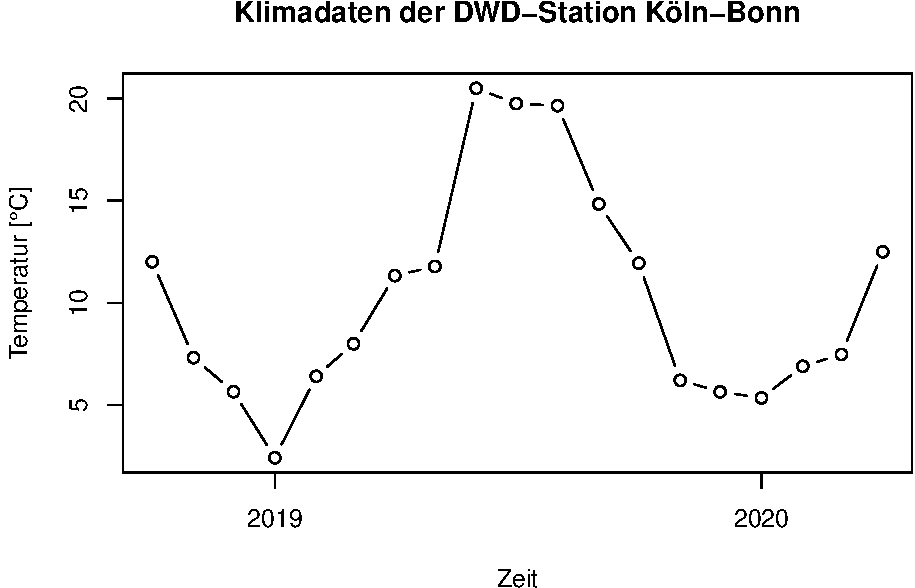
\includegraphics{datenanalyse_files/figure-latex/unnamed-chunk-22-1.pdf}

Die Funktion \texttt{plot} ist eine sogen. \emph{high-level} Grafikfunktion. Das bedeutet, dass sie alle Schritte des Plottens übernimmt: sie öffnet ein neues Grafikfenster (ein Device), berechnet die Größe der Plotfläche und der Ränder (s. unten), berechnet die Ausdehnung der Achsen und die beste Achseneinteilung und plottet Ihre Daten.

Daneben gibt es \emph{low-level} Grafikfunktionen, die nur in ein bestehendes Device plotten können. Wir wollen zu unserer Grafik nun die Minimum- und die Maximumtemperatur dazu plotten.

\begin{Shaded}
\begin{Highlighting}[]
\KeywordTok{plot}\NormalTok{(my_date, meteo}\OperatorTok{$}\NormalTok{MO_TT, }\DataTypeTok{type =} \StringTok{'b'}\NormalTok{, }\DataTypeTok{xlab =} \StringTok{'Zeit'}\NormalTok{, }\DataTypeTok{ylab =} \StringTok{'Temperatur [°C]'}\NormalTok{, }\DataTypeTok{main =} \StringTok{'Klimadaten der DWD-Station Köln-Bonn'}\NormalTok{)}

\CommentTok{# Minimumtemperatur in blau}
\KeywordTok{lines}\NormalTok{(my_date, meteo}\OperatorTok{$}\NormalTok{MO_TN, }\DataTypeTok{col =} \StringTok{'blue'}\NormalTok{)}

\CommentTok{# Maximumtemperatur in rot}
\KeywordTok{lines}\NormalTok{(my_date, meteo}\OperatorTok{$}\NormalTok{MO_TX, }\DataTypeTok{col =} \StringTok{'red'}\NormalTok{)}
\end{Highlighting}
\end{Shaded}

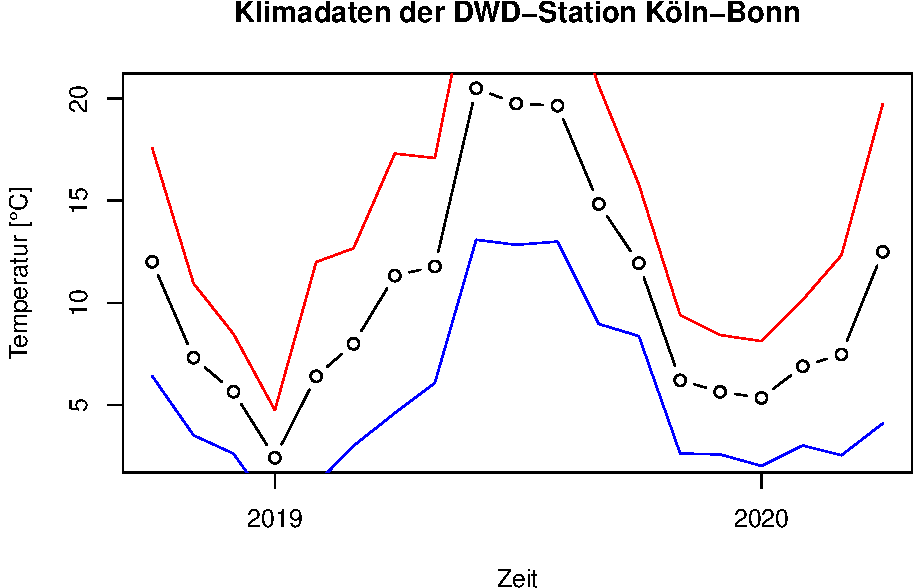
\includegraphics{datenanalyse_files/figure-latex/unnamed-chunk-23-1.pdf}

Dass \texttt{lines} nur eine \emph{low-level} Grafikfunktion ist, erkennen Sie daran, dass sie nicht in der Lage ist, den Bereich auf der y-Achse zu vergrößern, um alle Daten sichtbar zu machen. Das kann nur \texttt{plot}. Daher muss der Bereich bereits in \texttt{plot} richtig festgelegt werden. Das macht der Parameter \texttt{ylim}.

\begin{Shaded}
\begin{Highlighting}[]
\KeywordTok{plot}\NormalTok{(my_date, meteo}\OperatorTok{$}\NormalTok{MO_TT, }\DataTypeTok{type =} \StringTok{'b'}\NormalTok{, }\DataTypeTok{xlab =} \StringTok{'Zeit'}\NormalTok{, }\DataTypeTok{ylab =} \StringTok{'Temperatur [°C]'}\NormalTok{, }\DataTypeTok{main =} \StringTok{'Klimadaten der DWD-Station Köln-Bonn'}\NormalTok{, }\DataTypeTok{ylim =} \KeywordTok{c}\NormalTok{(}\DecValTok{0}\NormalTok{, }\DecValTok{30}\NormalTok{))}

\CommentTok{# Minimumtemperatur in rot}
\KeywordTok{lines}\NormalTok{(my_date, meteo}\OperatorTok{$}\NormalTok{MO_TN, }\DataTypeTok{col =} \StringTok{'blue'}\NormalTok{)}

\CommentTok{# Maximumtemperatur in blau}
\KeywordTok{lines}\NormalTok{(my_date, meteo}\OperatorTok{$}\NormalTok{MO_TX, }\DataTypeTok{col =} \StringTok{'red'}\NormalTok{)}
\end{Highlighting}
\end{Shaded}

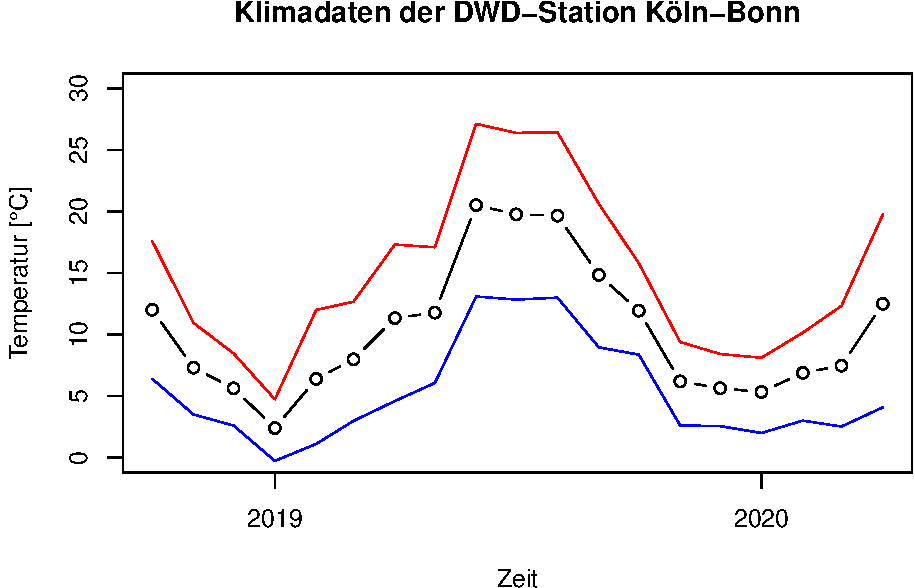
\includegraphics{datenanalyse_files/figure-latex/unnamed-chunk-24-1.pdf}

Wenn in einer Grafik mehrere Elemente dargestellt werden, benötigt man eine Legende. Das erledigt die * low-level* Grafikfunktion \texttt{legend}.

\begin{Shaded}
\begin{Highlighting}[]
\KeywordTok{plot}\NormalTok{(my_date, meteo}\OperatorTok{$}\NormalTok{MO_TT, }\DataTypeTok{type =} \StringTok{'b'}\NormalTok{, }\DataTypeTok{xlab =} \StringTok{'Zeit'}\NormalTok{, }\DataTypeTok{ylab =} \StringTok{'Temperatur [°C]'}\NormalTok{, }\DataTypeTok{main =} \StringTok{'Klimadaten der DWD-Station Köln-Bonn'}\NormalTok{, }\DataTypeTok{ylim =} \KeywordTok{c}\NormalTok{(}\DecValTok{0}\NormalTok{, }\DecValTok{30}\NormalTok{))}

\CommentTok{# Minimumtemperatur in rot}
\KeywordTok{lines}\NormalTok{(my_date, meteo}\OperatorTok{$}\NormalTok{MO_TN, }\DataTypeTok{col =} \StringTok{'blue'}\NormalTok{)}

\CommentTok{# Maximumtemperatur in blau}
\KeywordTok{lines}\NormalTok{(my_date, meteo}\OperatorTok{$}\NormalTok{MO_TX, }\DataTypeTok{col =} \StringTok{'red'}\NormalTok{)}

\KeywordTok{legend}\NormalTok{(}\StringTok{'topright'}\NormalTok{, }\DataTypeTok{legend =} \KeywordTok{c}\NormalTok{(}\StringTok{'Mittelwert'}\NormalTok{, }\StringTok{'Minimum'}\NormalTok{, }\StringTok{'Maximum'}\NormalTok{),}
       \DataTypeTok{col =} \KeywordTok{c}\NormalTok{(}\StringTok{'black'}\NormalTok{, }\StringTok{'red'}\NormalTok{, }\StringTok{'blue'}\NormalTok{), }
       \DataTypeTok{pch =} \KeywordTok{c}\NormalTok{(}\DecValTok{1}\NormalTok{, }\OtherTok{NA}\NormalTok{, }\OtherTok{NA}\NormalTok{),}
       \DataTypeTok{lty =} \DecValTok{1}\NormalTok{)}
\end{Highlighting}
\end{Shaded}

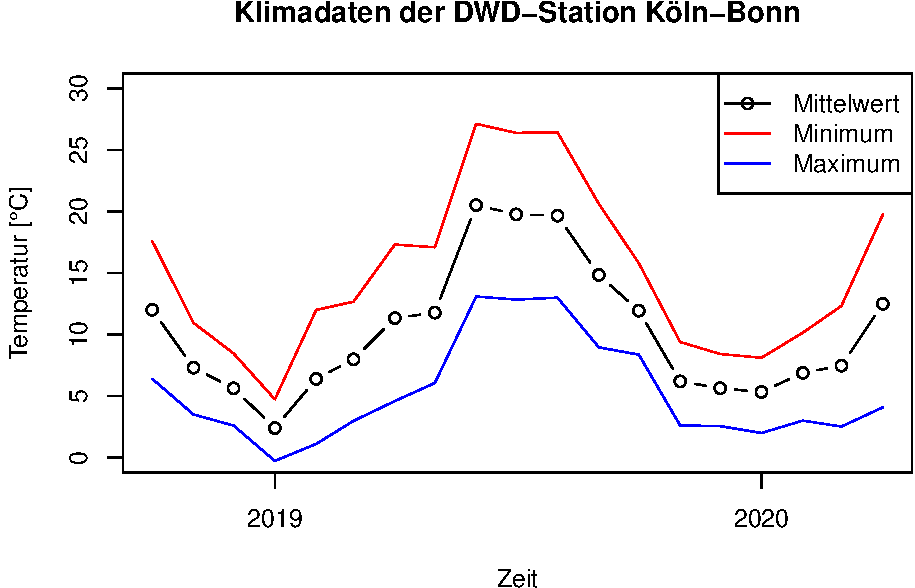
\includegraphics{datenanalyse_files/figure-latex/unnamed-chunk-25-1.pdf}

Der Parameter \texttt{lty} steht für \emph{line type} und die 1 bedeutet durchgezogene Linie. Mit \texttt{pch} legend wir die Art des Symbols fest; hier steht die 1 für das Standardsymbol ``offener Kreis''. Die Funktion \texttt{legend} hat viele Möglichkeiten und es lohnt sich, in die Hilfe zu sehen \texttt{?legend}.

\hypertarget{uxfcberblick-uxfcber-die-wichtigsten-high-level-und-low-level-grafikfunktionen}{%
\subsection{\texorpdfstring{Überblick über die wichtigsten \emph{high-level} und \emph{low-level} Grafikfunktionen}{Überblick über die wichtigsten high-level und low-level Grafikfunktionen}}\label{uxfcberblick-uxfcber-die-wichtigsten-high-level-und-low-level-grafikfunktionen}}

Die wichtigsten \emph{high-level} Grafikfunktionen nach \citet{Ligges2008}, verändert:

\begin{longtable}[]{@{}ll@{}}
\toprule
\begin{minipage}[b]{0.38\columnwidth}\raggedright
Funktion\strut
\end{minipage} & \begin{minipage}[b]{0.56\columnwidth}\raggedright
Beschreibung\strut
\end{minipage}\tabularnewline
\midrule
\endhead
\begin{minipage}[t]{0.38\columnwidth}\raggedright
\texttt{plot}\strut
\end{minipage} & \begin{minipage}[t]{0.56\columnwidth}\raggedright
kontextabhängig -- generische Funktion mit vielen Methoden\strut
\end{minipage}\tabularnewline
\begin{minipage}[t]{0.38\columnwidth}\raggedright
\texttt{barplot}\strut
\end{minipage} & \begin{minipage}[t]{0.56\columnwidth}\raggedright
Säulendiagramm\strut
\end{minipage}\tabularnewline
\begin{minipage}[t]{0.38\columnwidth}\raggedright
\texttt{boxplot}\strut
\end{minipage} & \begin{minipage}[t]{0.56\columnwidth}\raggedright
Boxplot\strut
\end{minipage}\tabularnewline
\begin{minipage}[t]{0.38\columnwidth}\raggedright
\texttt{contour}\strut
\end{minipage} & \begin{minipage}[t]{0.56\columnwidth}\raggedright
Höhenlinien-Plot\strut
\end{minipage}\tabularnewline
\begin{minipage}[t]{0.38\columnwidth}\raggedright
\texttt{coplot}\strut
\end{minipage} & \begin{minipage}[t]{0.56\columnwidth}\raggedright
Conditioning-Plots: Plots zweier Variablen aufgeteilt nach Werten einer dritten\strut
\end{minipage}\tabularnewline
\begin{minipage}[t]{0.38\columnwidth}\raggedright
\texttt{curve}\strut
\end{minipage} & \begin{minipage}[t]{0.56\columnwidth}\raggedright
Funktionen zeichnen\strut
\end{minipage}\tabularnewline
\begin{minipage}[t]{0.38\columnwidth}\raggedright
\texttt{dotchart}\strut
\end{minipage} & \begin{minipage}[t]{0.56\columnwidth}\raggedright
Dotplots (nach Cleveland)\strut
\end{minipage}\tabularnewline
\begin{minipage}[t]{0.38\columnwidth}\raggedright
\texttt{hist}\strut
\end{minipage} & \begin{minipage}[t]{0.56\columnwidth}\raggedright
Histogramm\strut
\end{minipage}\tabularnewline
\begin{minipage}[t]{0.38\columnwidth}\raggedright
\texttt{image}\strut
\end{minipage} & \begin{minipage}[t]{0.56\columnwidth}\raggedright
Bilder (3. Dimension als Farbe)\strut
\end{minipage}\tabularnewline
\begin{minipage}[t]{0.38\columnwidth}\raggedright
\texttt{mosaicplot}\strut
\end{minipage} & \begin{minipage}[t]{0.56\columnwidth}\raggedright
Mosaikplots (kategorielle Daten)\strut
\end{minipage}\tabularnewline
\begin{minipage}[t]{0.38\columnwidth}\raggedright
\texttt{pairs}\strut
\end{minipage} & \begin{minipage}[t]{0.56\columnwidth}\raggedright
Streudiagramm-Matrix\strut
\end{minipage}\tabularnewline
\begin{minipage}[t]{0.38\columnwidth}\raggedright
\texttt{persp}\strut
\end{minipage} & \begin{minipage}[t]{0.56\columnwidth}\raggedright
perspektivische Flächen\strut
\end{minipage}\tabularnewline
\begin{minipage}[t]{0.38\columnwidth}\raggedright
\texttt{qqnorm} und \texttt{qqplot}\strut
\end{minipage} & \begin{minipage}[t]{0.56\columnwidth}\raggedright
QQ--Plot\strut
\end{minipage}\tabularnewline
\bottomrule
\end{longtable}

Die wichtigsten \emph{low-level} Grafikfunktionen nach \citet{Ligges2008}, verändert:

\begin{longtable}[]{@{}ll@{}}
\toprule
\begin{minipage}[b]{0.38\columnwidth}\raggedright
Funktion\strut
\end{minipage} & \begin{minipage}[b]{0.56\columnwidth}\raggedright
Beschreibung\strut
\end{minipage}\tabularnewline
\midrule
\endhead
\begin{minipage}[t]{0.38\columnwidth}\raggedright
\texttt{abline}\strut
\end{minipage} & \begin{minipage}[t]{0.56\columnwidth}\raggedright
Fügt eine Linie hinzu; diese kann horizontal, vertikal oder über Steigung und Achsenabschnitt definiert werden\strut
\end{minipage}\tabularnewline
\begin{minipage}[t]{0.38\columnwidth}\raggedright
\texttt{arrows}\strut
\end{minipage} & \begin{minipage}[t]{0.56\columnwidth}\raggedright
Pfeile\strut
\end{minipage}\tabularnewline
\begin{minipage}[t]{0.38\columnwidth}\raggedright
\texttt{axis}\strut
\end{minipage} & \begin{minipage}[t]{0.56\columnwidth}\raggedright
Achsen\strut
\end{minipage}\tabularnewline
\begin{minipage}[t]{0.38\columnwidth}\raggedright
\texttt{grid}\strut
\end{minipage} & \begin{minipage}[t]{0.56\columnwidth}\raggedright
Gitternetz\strut
\end{minipage}\tabularnewline
\begin{minipage}[t]{0.38\columnwidth}\raggedright
\texttt{legend}\strut
\end{minipage} & \begin{minipage}[t]{0.56\columnwidth}\raggedright
Legende\strut
\end{minipage}\tabularnewline
\begin{minipage}[t]{0.38\columnwidth}\raggedright
\texttt{lines}\strut
\end{minipage} & \begin{minipage}[t]{0.56\columnwidth}\raggedright
Linien (schrittweise)\strut
\end{minipage}\tabularnewline
\begin{minipage}[t]{0.38\columnwidth}\raggedright
\texttt{mtext}\strut
\end{minipage} & \begin{minipage}[t]{0.56\columnwidth}\raggedright
Text in den Rändern\strut
\end{minipage}\tabularnewline
\begin{minipage}[t]{0.38\columnwidth}\raggedright
\texttt{plot.new}\strut
\end{minipage} & \begin{minipage}[t]{0.56\columnwidth}\raggedright
Grafik initialisieren\strut
\end{minipage}\tabularnewline
\begin{minipage}[t]{0.38\columnwidth}\raggedright
\texttt{plot.window}\strut
\end{minipage} & \begin{minipage}[t]{0.56\columnwidth}\raggedright
Koordinatensystem initialisieren\strut
\end{minipage}\tabularnewline
\begin{minipage}[t]{0.38\columnwidth}\raggedright
\texttt{points}\strut
\end{minipage} & \begin{minipage}[t]{0.56\columnwidth}\raggedright
Punkte\strut
\end{minipage}\tabularnewline
\begin{minipage}[t]{0.38\columnwidth}\raggedright
\texttt{polygon}\strut
\end{minipage} & \begin{minipage}[t]{0.56\columnwidth}\raggedright
(ausgefüllte) Polygone\strut
\end{minipage}\tabularnewline
\begin{minipage}[t]{0.38\columnwidth}\raggedright
\texttt{pretty}\strut
\end{minipage} & \begin{minipage}[t]{0.56\columnwidth}\raggedright
berechnet ``hübsche'' Einteilung der Achsen\strut
\end{minipage}\tabularnewline
\begin{minipage}[t]{0.38\columnwidth}\raggedright
\texttt{segments}\strut
\end{minipage} & \begin{minipage}[t]{0.56\columnwidth}\raggedright
Linien (vektorwertig)\strut
\end{minipage}\tabularnewline
\begin{minipage}[t]{0.38\columnwidth}\raggedright
\texttt{text}\strut
\end{minipage} & \begin{minipage}[t]{0.56\columnwidth}\raggedright
Text\strut
\end{minipage}\tabularnewline
\begin{minipage}[t]{0.38\columnwidth}\raggedright
\texttt{title}\strut
\end{minipage} & \begin{minipage}[t]{0.56\columnwidth}\raggedright
Beschriftung\strut
\end{minipage}\tabularnewline
\bottomrule
\end{longtable}

\hypertarget{tuning-mit-par}{%
\section{\texorpdfstring{Tuning mit \texttt{par}}{Tuning mit par}}\label{tuning-mit-par}}

Zur Vertiefung dieses Kapitels, empfehle ich \citet{Ligges2008}, Kapitel 8.1.3.

Die Grafikebene in R ist aufgeteilt in drei Regionen (Abbildung \ref{fig:aufteilung}) und hat innere und äußere Ränder. Die Ränder werden von unten im Gegenuhrzeigersinn durchnummeriert.

\begin{figure}
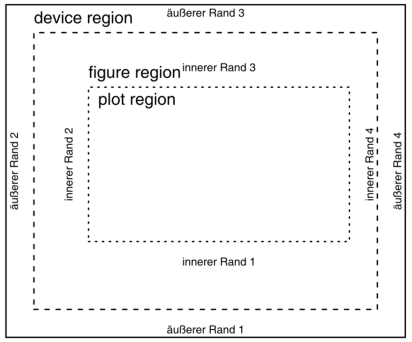
\includegraphics[width=0.8\linewidth]{Regionen_und_Raender} \caption{Aufteilung der Grafikfläche [@Ligges2008].}\label{fig:aufteilung}
\end{figure}

Mit der Funktion \texttt{par} lassen sich sehr viele Einstellung der Grafik verändern. Viele Einstellungen übergibt die Funktion \texttt{plot} selbständig an \texttt{par}, zu.B. \texttt{log} (Logarithmieren der Achsen), \texttt{cex} (Größe eines Punkts) oder \texttt{col} (Farbe). Andere können aber nur durch Aufrufen der Funktion \texttt{par} verändert werden. Dazu gehören die inneren Ränder \texttt{mar} und die äußeren Ränder \texttt{oma}, die Aufteilung der Grafikebene mit \texttt{mfrow} oder \texttt{mfcol}.

\begin{rmdalert}
Richtige Benutzung von \texttt{par}:

\begin{itemize}
\tightlist
\item
  Parameter setzen: \texttt{op\ \textless{}-\ par(\ ...\ )}
\item
  plotten
\item
  Parameter auf Standard zurück setzen: \texttt{par(op)}
\end{itemize}
\end{rmdalert}

Die Zuweisung \texttt{op\ \textless{}-\ par(\ ...\ )} speichert die Standardeinstellungen im Objekt \texttt{par}, bevor Sie sie ändern. Der Aufruf \texttt{par(op)} setzt Ihre Änderungen zurück. Das ist sehr praktisch, wenn Sie z.B. die Aufteilung der Grafikebene nicht mehr benötigen. Wenn Sie die Parameter nicht zurücksetzen, bleiben diese bestehen, bis das Grafikfenster geschlossen wird (z.B. mit \texttt{dev.off()}).

Um die Ränder zu verändern, rufen wir \texttt{par} auf und beschneiden die Ränder, damit Sie den Unterschied erkennen können.

\begin{Shaded}
\begin{Highlighting}[]
\NormalTok{op <-}\StringTok{ }\KeywordTok{par}\NormalTok{(}\DataTypeTok{mar =} \KeywordTok{c}\NormalTok{(}\DecValTok{1}\NormalTok{, }\DecValTok{1}\NormalTok{, }\DecValTok{1}\NormalTok{, }\DecValTok{1}\NormalTok{))}
\KeywordTok{plot}\NormalTok{(my_date, meteo}\OperatorTok{$}\NormalTok{MO_TT, }\DataTypeTok{type =} \StringTok{'b'}\NormalTok{, }\DataTypeTok{xlab =} \StringTok{'Zeit'}\NormalTok{, }\DataTypeTok{ylab =} \StringTok{'Temperatur [°C]'}\NormalTok{, }\DataTypeTok{main =} \StringTok{'Klimadaten der DWD-Station Köln-Bonn'}\NormalTok{, }\DataTypeTok{ylim =} \KeywordTok{c}\NormalTok{(}\DecValTok{0}\NormalTok{, }\DecValTok{30}\NormalTok{))}

\CommentTok{# Minimumtemperatur in rot}
\KeywordTok{lines}\NormalTok{(my_date, meteo}\OperatorTok{$}\NormalTok{MO_TN, }\DataTypeTok{col =} \StringTok{'blue'}\NormalTok{)}

\CommentTok{# Maximumtemperatur in blau}
\KeywordTok{lines}\NormalTok{(my_date, meteo}\OperatorTok{$}\NormalTok{MO_TX, }\DataTypeTok{col =} \StringTok{'red'}\NormalTok{)}
\end{Highlighting}
\end{Shaded}

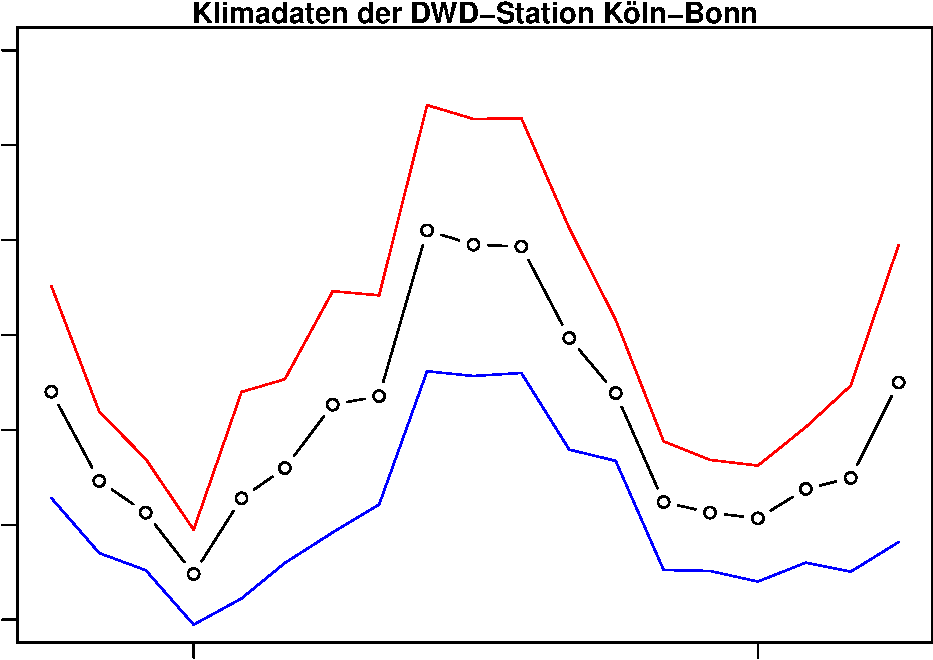
\includegraphics{datenanalyse_files/figure-latex/unnamed-chunk-27-1.pdf}

Die Achsenbeschriftungen und die Zahlen haben jetzt nicht mehr genug Platz und verschwinden. Die Größe der Ränder wird in Zeilen angegeben, ist also relativ zur Gesamtgröße. Die Standardeinstellung ist \texttt{c(5,\ 4,\ 4,\ 2)\ +\ 0.1}.

Einige häufig genutzte Argumente in Grafikfunktionen und in \texttt{par} \citep[nach][verändert]{Ligges2008}. Schlagen Sie die Erklärungen dazu immer in \texttt{?par} oder \texttt{?plot} nach.

\begin{longtable}[]{@{}ll@{}}
\toprule
Funktion & Beschreibung\tabularnewline
\midrule
\endhead
\texttt{axes} & Achsen sollen (nicht) eingezeichnet werden\tabularnewline
\texttt{bg} & Hintergrundfarbe\tabularnewline
\texttt{cex} & Größe eines Punktes bzw. Buchstaben\tabularnewline
\texttt{col} & Farben\tabularnewline
\texttt{las} & Ausrichtung der Achsenbeschriftung\tabularnewline
\texttt{log} & Logarithmierte Darstellung\tabularnewline
\texttt{lty}, \texttt{lwd} & Linientyp (gestrichelt, \ldots{}) und Linienbreite\tabularnewline
\texttt{main} & Überschrift\tabularnewline
\texttt{mar} & Größe der inneren Ränder für Achsenbeschriftung etc.\tabularnewline
\texttt{mfcol}, \texttt{mfrow} & mehrere Grafiken in einem Bild\tabularnewline
\texttt{pch} & Symbol für einen Punkt\tabularnewline
\texttt{type} & Typ (l für Linie, p für Punkt, b für beides, n für nichts)\tabularnewline
\texttt{usr} & Ausmaße der Achsen auslesen\tabularnewline
\texttt{xlab}, \texttt{ylab} & x-/y-Achsenbeschriftung\tabularnewline
\texttt{xlim}, \texttt{ylim} & zu plottender Bereich in x-/y- Richtung\tabularnewline
\texttt{xpd} & in die Ränder hinein zeichnen\tabularnewline
\bottomrule
\end{longtable}

\hypertarget{inhalt-der-live-einfuxfchrung-2}{%
\section{Inhalt der live Einführung}\label{inhalt-der-live-einfuxfchrung-2}}

\begin{itemize}
\tightlist
\item
  \texttt{plot}, \texttt{barplot}, \texttt{mfrow}
\item
  Aufgaben \ref{wahlbeteiligung}, \ref{zweitstimme} und \ref{zweigrafiken}.
\item
  Speichern als pdf
\end{itemize}

\hypertarget{aufgabensammlung}{%
\chapter{Aufgabensammlung}\label{aufgabensammlung}}

\hypertarget{erste-schritte}{%
\section{Erste Schritte}\label{erste-schritte}}

\hypertarget{ars-haushaltsbuch}{%
\subsection{Ars Haushaltsbuch}\label{ars-haushaltsbuch}}

Der angehende Datenanalyst Ar Stat möchte dem Rat seiner Mutter folgen und ein Haushaltsbuch anlegen. Als erstes möchte er sich einen Überblick über seine Ausgaben in der Uni-Mensa verschaffen und erstellt die folgende Tabelle:

\begin{table}

\caption{\label{tab:unnamed-chunk-29}Ars Mensaausgaben}
\centering
\begin{tabular}[t]{lr}
\toprule
Wochentag & Ausgaben\\
\midrule
Montag & 2,57\\
Dienstag & 2,90\\
Mittwoch & 2,73\\
Donnerstag & 3,23\\
Freitag & 3,90\\
\bottomrule
\end{tabular}
\end{table}

\begin{enumerate}
\def\labelenumi{\arabic{enumi}.}
\tightlist
\item
  Wie viel hat Ar insgesamt in der Woche ausgegeben?
\item
  Wie viel hat er im Schnitt pro Tag ausgegeben?
\item
  Wie stark schwanken seine Ausgaben?
\end{enumerate}

Leider hat Ar sich beim übertragen der Daten vertippt. Er hat am Dienstag seine Freundin zum Essen eingeladen und 7,95 € statt 2,90 € ausgegeben.

\begin{enumerate}
\def\labelenumi{\arabic{enumi}.}
\setcounter{enumi}{3}
\tightlist
\item
  Korrigieren Sie Ars Fehler.
\item
  Wie verändern sich die Ergebnisse aus den Teilaufgaben 1 bis 3 Warum?
\end{enumerate}

\hypertarget{daten-in-r}{%
\section{Daten in R}\label{daten-in-r}}

\hypertarget{bestandesaufnahme}{%
\subsection{Bestandesaufnahme im Wald}\label{bestandesaufnahme}}

Ar Stat arbeitet als HiWi in der AG Ökosystemforschung und soll im Nationalpark Eifel eine Bestandsaufnahme durchführen (d.h. Baumhöhen und -durchmesser vermessen). Er notiert den BHD (Brusthöhendurchmesser) und die Art der Bäume.

\begin{enumerate}
\def\labelenumi{\arabic{enumi}.}
\tightlist
\item
  Lesen Sie den Datensatz \texttt{BHD.txt} ein und ordnen Sie ihn der Variable \texttt{BHD} zu.
\item
  Erstellen Sie einen Vektor \texttt{a} mit Baumnummern. Von welcher Art sind die Elemente des Vektors \texttt{a}?
\item
  Fügen Sie die Datensätze \texttt{BHD} und \texttt{a} zu einem \texttt{data.frame} zusammen und benennen Sie die Spalten sinnvoll.
\item
  Löschen Sie den Vektor \texttt{a}.
\item
  Lesen Sie den Datensatz \texttt{Art.txt} ein und ordnen Sie ihn der Variablen \texttt{art} zu.
\item
  Fügen Sie die Art in den \texttt{data.frame} ein.
\item
  Erstellen Sie eine Tabelle mit der Anzahl der jeweiligen Arten. Nutzen Sie die Funktion \texttt{table}.
\item
  Speichern Sie die Tabelle mit \texttt{write.table}.
\end{enumerate}

\hypertarget{daten-visualisieren-teil-i-fokus-auf-r}{%
\section{Daten visualisieren, Teil I: Fokus auf R}\label{daten-visualisieren-teil-i-fokus-auf-r}}

\hypertarget{wahlbeteiligung}{%
\subsection{Wahlbeteiligung bei der Bundestagswahl 2017}\label{wahlbeteiligung}}

Bauen Sie die Grafiken aus der Einführung nach (Abbildung \ref{fig:wahlbeteiligung}).

\begin{figure}
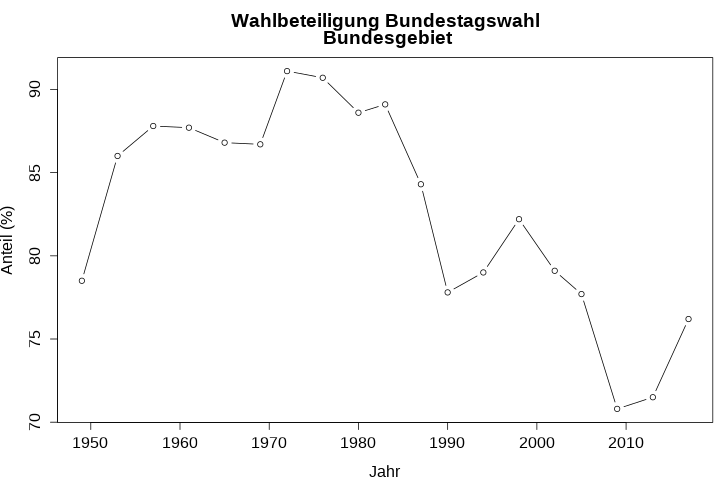
\includegraphics[width=1\linewidth]{Wahlbeteiligung} \caption{Wahlbeteiligung bei den Bundestagswahlen. Quelle: Der Bundeswahlleiter.}\label{fig:wahlbeteiligung}
\end{figure}

\begin{enumerate}
\def\labelenumi{\arabic{enumi}.}
\tightlist
\item
  Lesen Sie den Datensatz \texttt{Wahlbeteiligung.csv} in R ein und ordnen Sie ihn dem Objekt \texttt{bet} zu. Der Datensatz hat einen \emph{header} und haben einen Strichpunkt als Spaltentrenner.
\item
  Sehen Sie sich die Struktur und die ersten und letzten 6 Zeilen des Datensatzes an.
\item
  Stellen Sie die Wahlbeteiligung als Funktion der Zeit in einem Streudiagramm dar. Wählen Sie die passende Darstellungsform \texttt{type}.
\item
  Beschriften Sie die Grafik.
\item
  Speichern Sie die Grafik als pdf ab.
\end{enumerate}

\hypertarget{zweitstimme}{%
\subsection{Zweitstimme bei der Bundestagswahl 2017}\label{zweitstimme}}

Bauen Sie die Grafiken aus der Einführung nach (Abbildung \ref{fig:zweitstimme}).

\begin{figure}
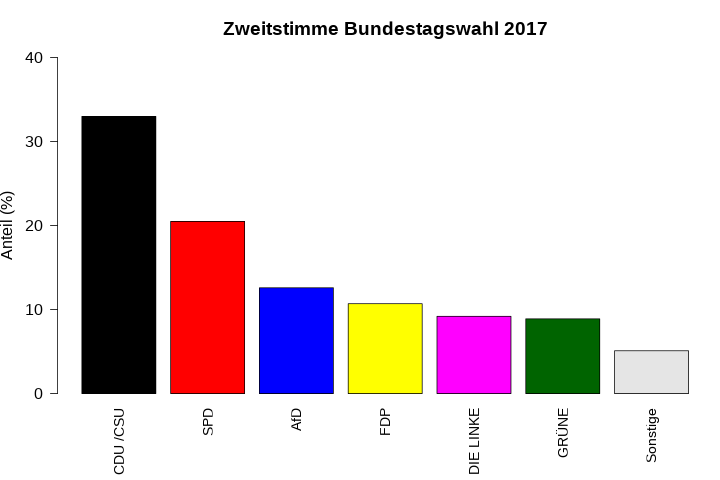
\includegraphics[width=1\linewidth]{Zweitstimme} \caption{Zweitstimme bei der Bundestagswahl 2017. Quelle: Der Bundeswahlleiter.}\label{fig:zweitstimme}
\end{figure}

\begin{enumerate}
\def\labelenumi{\arabic{enumi}.}
\tightlist
\item
  Lesen Sie den Datensatz \texttt{Zweitstimme.csv} in R ein und ordnen Sie ihn dem Objekt \texttt{zweit} zu. Der Datensatz hat einen \emph{header} und haben einen Strichpunkt als Spaltentrenner.
\item
  Sehen Sie sich die Struktur und die ersten und letzten 6 Zeilen des Datensatzes an.
\item
  Stellen Sie die die Zweitstimmen pro Partei in einem Säulendiagramm dar. Sortieren Sie die Zweitstimmen in absteigender Reihenfolge.
\item
  Beschriften Sie die Grafik.
\item
  Speichern Sie die Grafik als pdf ab.
\end{enumerate}

\hypertarget{zweigrafiken}{%
\subsection{Ergebnisse der Bundestagswahl in einer Grafik}\label{zweigrafiken}}

Stellen Sie beide Grafiken nebeneinander dar wie in Abbildung (\ref{zweigrafiken}) gezeigt.

\begin{figure}
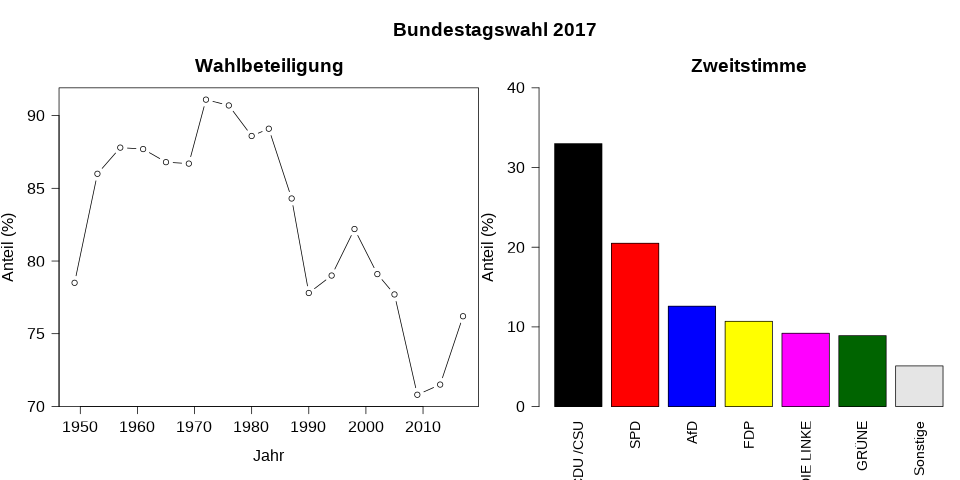
\includegraphics[width=1\linewidth]{Zwei_grafiken} \caption{Ergebnisse der Bundestagswahl 2017. Quelle: Der Bundeswahlleiter.}\label{fig:zweigrafiken}
\end{figure}

\hypertarget{weisserrand}{%
\subsection{Einen zu großen weißen Rand vermeiden}\label{weisserrand}}

Bei Berichten haben Abbildungen meistens keine Überschrift, da alles in der Bildunterschrift erklärt wird. Wenn man die Überschrift beim plotten weglässt, die Standardeinstellungen für die Ränder aber beibehält, entsteht ein zu großer weißer Rand um die Grafik. Diesen wollen wir nun abschalten.

\begin{enumerate}
\def\labelenumi{\arabic{enumi}.}
\tightlist
\item
  Kopieren Sie den Code zum Plotten der Temperaturen aus dem Kapitel \ref{visualisieren}.
\item
  Stellen Sie oben und rechts einen Rand von 0.1 Zeilen ein.
\item
  Speichern Sie die Grafik als pdf ab.
\end{enumerate}

\hypertarget{spielen-mit-der-funktion-par}{%
\subsection{\texorpdfstring{Spielen mit der Funktion \texttt{par}}{Spielen mit der Funktion par}}\label{spielen-mit-der-funktion-par}}

Setzen Sie die Übung \ref{weisserrand} fort. Denken Sie an den richtigen Aufruf mit der Zuweisung von \texttt{op\ \textless{}-\ par(\ ...\ )}!

\begin{enumerate}
\def\labelenumi{\arabic{enumi}.}
\tightlist
\item
  Probieren Sie die Größeneinstellung \texttt{cex\ =\ 2} in \texttt{plot} aus. Testen Sie unterschiedliche Werte.
\item
  Probieren Sie die Einstellungen \texttt{cex.axis}, \texttt{cex.lab} und \texttt{cex.main} in \texttt{par} aus.
\item
  Probieren Sie die Einstellung \texttt{col} in \texttt{plot} aus.
\item
  Probieren Sie die Einstellungen \texttt{col.axis}, \texttt{col.lab} und \texttt{col.main} aus.
\item
  Probieren Sie die Schrifteinstellungen aus. Dazu stellen Sie den Parameter \texttt{family} in \texttt{par} auf ``serif'', ``sans'' oder ``mono''.
\item
  Probieren Sie die Parameter \texttt{font.lab\ =\ 2} und \texttt{font.axis\ =\ 2} direkt in \texttt{plot} aus. Zahlen 1 bis 5 stehen jeweils für normal, fett, kursiv, fett-kursiv und symbolisch.
\end{enumerate}

\hypertarget{eigene-funktionen-schreiben}{%
\section{Eigene Funktionen schreiben}\label{eigene-funktionen-schreiben}}

\hypertarget{r-hausaufgaben}{%
\subsection{R-Hausaufgaben}\label{r-hausaufgaben}}

An dem Kurs ``Einführung in R'' nehmen 49 Studierende teil. Der Leistungsnachweis besteht aus Hausaufgaben, die insgesamt mit 100 Punkten bewertet werden. Ab 50 Punkten gilt der Kurs als bestanden.

\begin{enumerate}
\def\labelenumi{\arabic{enumi}.}
\tightlist
\item
  Lesen Sie den Datensatz \texttt{R-HAs.txt}, der die Endpunkte enthält, ein.
\item
  Ermitteln Sie, wie viele Teilnehmer bestanden und wie viele nicht bestanden haben.
\end{enumerate}

\hypertarget{fledermuxe4use-die-zweite}{%
\subsection{Fledermäuse, die Zweite}\label{fledermuxe4use-die-zweite}}

Wir beschäftigen uns erneut mit den Fledermäusen.

\begin{enumerate}
\def\labelenumi{\arabic{enumi}.}
\tightlist
\item
  Lesen Sie den korrigierten(!) Datensatz \textbackslash{}texttt\{Fledermaus\_cor.txt\} ein.
\item
  Schreiben Sie eine Funktion, die den Entwicklungsstand der Tiere klassifiziert. Nutzen Sie dazu die ad hoc Regel: Individuum \textless{} 5 cm ist ein Jungtier, sonst erwachsen.
\item
  Erstellen Sie eine ordinal-skalierte Variable \texttt{alter} mit dem Entwicklungsstand der Tiere.
\item
  Schreiben Sie eine Funktion, die die Mittelwerte der Größe für weibliche und männliche Individuen berechnet.
\item
  Berechnen Sie die Mittelwerte der Größe und runden Sie auf 2 Nachkommastellen.
\end{enumerate}

\hypertarget{unfaire-klausur}{%
\subsection{Unfaire Klausur?}\label{unfaire-klausur}}

Ar belegt im 4. Semester die Veranstaltung ``Spaß mit R''. Bei der Klausur gibt es 2 Aufgabengruppen mit jeweils 60 Punkten. Aufgabengruppe 1 wird an Studierende auf ungeraden Sitzplätzen und Aufgabengruppe 2 an Studierende auf geraden Sitzplätzen ausgegeben.

\begin{enumerate}
\def\labelenumi{\arabic{enumi}.}
\tightlist
\item
  Lesen Sie den Datensatz \texttt{Klausurpunkte.txt} ein.
\item
  Überprüfen Sie Ars Vermutung, dass die Aufgabengruppe 1 im Schnitt leichter war als Aufgabengruppe 2 (d.h. in der Gruppe 1 im Schnitt mehr Punkte erzielt wurden).
\end{enumerate}

\hypertarget{daten-visualisieren-teil-ii-fokus-auf-daten}{%
\section{Daten visualisieren, Teil II: Fokus auf Daten}\label{daten-visualisieren-teil-ii-fokus-auf-daten}}

\hypertarget{zeitreihen-aus-der-langen-bramke-harz}{%
\subsection{Zeitreihen aus der Langen Bramke (Harz)}\label{zeitreihen-aus-der-langen-bramke-harz}}

Im Harz wurden über eine längere Zeit Niederschlag, Abfluss und Temperatur gemessen.

\begin{enumerate}
\def\labelenumi{\arabic{enumi}.}
\tightlist
\item
  Laden Sie den Datensatz \texttt{Data.dat}.
\item
  Stellen Sie die Temperatur in einem Streudiagramm dar. Welche Darstellungsart (Argument \texttt{type} in \texttt{plot}) erscheint Ihnen am sinnvollsten?
\item
  Beschriften Sie die Graphik und fügen Sie einen Titel hinzu.
\item
  Speichern Sie die Graphik als pdf ab.
\item
  Stellen Sie die Niederschläge in einem Diagramm dar. Wählen Sie einen geeigneten Darstellungstyp mit \texttt{type} (Tipp: geben Sie für die Hilfe \texttt{?plot} in die Console ein).
\end{enumerate}

\hypertarget{temperatur-datensatz}{%
\subsection{Temperatur-Datensatz}\label{temperatur-datensatz}}

\begin{enumerate}
\def\labelenumi{\arabic{enumi}.}
\tightlist
\item
  Laden Sie den Temperatur-Datensatz aus \citet{Zuur2009a}.
\item
  Berechnen Sie die Monatsmittelwerte für alle Stationen, sowie die Standardabweichungen.
\item
  Stellen Sie die Monatsmittel der Temperatur in einem Säulendiagramm dar.
\item
  Beschriften Sie die Graphik sinnvoll.
\item
  Fügen Sie die Standardabweichungen zu den einzelnen Balken hinzu.
\end{enumerate}

\hypertarget{artenvielfalt-in-grasluxe4ndern}{%
\subsection{Artenvielfalt in Grasländern}\label{artenvielfalt-in-grasluxe4ndern}}

Sie erhalten Daten aus dem Grasland-Monitoring im Yellowstone Nationalpark und dem National Bison Range (USA). Das Ziel des Monitorings ist die Untersuchung möglicher Änderungen der Biodiversität und des Zusammenhang mit Umweltfaktoren. Biodiversität wurde durch die Anzahl unterschiedlicher Arten quantifiziert. Insgesamt haben die Forscher ca. 90 Arten in 8 Transekten kartiert. Die Aufnahmen wurden alle 4 bis 10 Jahre wiederholt. Insgesamt liegen 58 Beobachtungen vor. Die Daten sind in der Datei \texttt{Vegetation2.xls} gespeichert.

\begin{enumerate}
\def\labelenumi{\arabic{enumi}.}
\item
  Laden Sie den Datensatz in R und sehen Sie sich das Ergebnis genau mit \texttt{str}, \texttt{head} und \texttt{tail} an. Diese Aufgabe dient dazu, das Einlesen von Excel-Dateien zu erarbeiten. Tipp: eine mögliche Bibliothek, die dabei helfen kann, wäre \texttt{xlsx}.
\item
  Berechnen Sie den Mittelwert und die Standardabweichung der Artenzahl (Variable \texttt{R}) pro Transekt.
\item
  Plotten Sie die Artenzahl gegen die Variable \texttt{BARESOIL} (Anteil von unbewachsenem Boden).
\item
  Benutzen Sie unterschiedliche Symbole pro Transekt, erstellen Sie eine Legende.
\item
  Beschriften Sie die Graphik sinnvoll und speichern Sie sie als pdf ab, ohne die Maus zu benutzen.
\end{enumerate}

\hypertarget{tracerversuche}{%
\subsection{Tracerversuche}\label{tracerversuche}}

Im Waldstein wurden Tracerversuche mit dem Farbstoff Brilliant Blue durchgeführt und die gefärbten Bodenprofile \emph{binärisiert} (d.h. in ein schwarz-weiß Bild umgewandelt). Schwarze Pixels stellen gefärbten Boden und weiße ungefärbten dar. Aus diesen Binärbildern wurde anschließend eine Reihe von Kenngrößen berechnet.

\begin{enumerate}
\def\labelenumi{\arabic{enumi}.}
\tightlist
\item
  Lesen Sie die Datei \textbackslash{}texttt\{Waldstein2005\_ind.txt\} ein. Die Tiefe eines Profils ist 579 Pixel und es liegen 6 Profile untereinander in der Spalte d.
\item
  Berechnen Sie die 5\%, 50\% und 95\% Quantile des Färbeanteils (Index d) der 6 Profile.
\item
  Stellen Sie den Median des Anteils der Färbung mit der Tiefe dar und fügen Sie die Quantile als transparente Fläche hinzu (Tipp: \texttt{polygon}).
\end{enumerate}

\hypertarget{effizientes-programmieren}{%
\section{Effizientes Programmieren}\label{effizientes-programmieren}}

\hypertarget{lagerungsdichten}{%
\subsection{Lagerungsdichten}\label{lagerungsdichten}}

Auf 10 verschiedenen landwirtschaftlichen Feldern wurden im Oberboden je 25 Stechzylinder entnommen.

\begin{enumerate}
\def\labelenumi{\arabic{enumi}.}
\tightlist
\item
  Lesen Sie den Datensatz \texttt{Bodendaten.txt} ein.
\item
  Bestimmen Sie die mittlere Lagerungsdichte pro Feld.
\end{enumerate}

\hypertarget{temperatur-datensatz-revisited}{%
\subsection{Temperatur-Datensatz, revisited}\label{temperatur-datensatz-revisited}}

\begin{enumerate}
\def\labelenumi{\arabic{enumi}.}
\tightlist
\item
  Laden Sie den Temperatur-Datensatz aus \citet{Zuur2009a}, Datei \texttt{Temperatur.csv}.
\item
  Berechnen Sie die Jahresmittelwerte je Station. (Tipp: Hilfe von \texttt{tapply} genau lesen!)
\end{enumerate}

\hypertarget{refs}{}

\bibliography{book.bib,packages.bib}

\end{document}
